\documentclass[]{article}
\usepackage{lmodern}
\usepackage{amssymb,amsmath}
\usepackage{ifxetex,ifluatex}
\usepackage{fixltx2e} % provides \textsubscript
\ifnum 0\ifxetex 1\fi\ifluatex 1\fi=0 % if pdftex
  \usepackage[T1]{fontenc}
  \usepackage[utf8]{inputenc}
\else % if luatex or xelatex
  \ifxetex
    \usepackage{mathspec}
  \else
    \usepackage{fontspec}
  \fi
  \defaultfontfeatures{Ligatures=TeX,Scale=MatchLowercase}
\fi
% use upquote if available, for straight quotes in verbatim environments
\IfFileExists{upquote.sty}{\usepackage{upquote}}{}
% use microtype if available
\IfFileExists{microtype.sty}{%
\usepackage{microtype}
\UseMicrotypeSet[protrusion]{basicmath} % disable protrusion for tt fonts
}{}
\usepackage[margin=1in]{geometry}
\usepackage{hyperref}
\hypersetup{unicode=true,
            pdftitle={Find-A-Gene - A. Geffre - BGGN213 Spring 2019},
            pdfauthor={A. C. Geffre},
            pdfborder={0 0 0},
            breaklinks=true}
\urlstyle{same}  % don't use monospace font for urls
\usepackage{color}
\usepackage{fancyvrb}
\newcommand{\VerbBar}{|}
\newcommand{\VERB}{\Verb[commandchars=\\\{\}]}
\DefineVerbatimEnvironment{Highlighting}{Verbatim}{commandchars=\\\{\}}
% Add ',fontsize=\small' for more characters per line
\usepackage{framed}
\definecolor{shadecolor}{RGB}{248,248,248}
\newenvironment{Shaded}{\begin{snugshade}}{\end{snugshade}}
\newcommand{\KeywordTok}[1]{\textcolor[rgb]{0.13,0.29,0.53}{\textbf{#1}}}
\newcommand{\DataTypeTok}[1]{\textcolor[rgb]{0.13,0.29,0.53}{#1}}
\newcommand{\DecValTok}[1]{\textcolor[rgb]{0.00,0.00,0.81}{#1}}
\newcommand{\BaseNTok}[1]{\textcolor[rgb]{0.00,0.00,0.81}{#1}}
\newcommand{\FloatTok}[1]{\textcolor[rgb]{0.00,0.00,0.81}{#1}}
\newcommand{\ConstantTok}[1]{\textcolor[rgb]{0.00,0.00,0.00}{#1}}
\newcommand{\CharTok}[1]{\textcolor[rgb]{0.31,0.60,0.02}{#1}}
\newcommand{\SpecialCharTok}[1]{\textcolor[rgb]{0.00,0.00,0.00}{#1}}
\newcommand{\StringTok}[1]{\textcolor[rgb]{0.31,0.60,0.02}{#1}}
\newcommand{\VerbatimStringTok}[1]{\textcolor[rgb]{0.31,0.60,0.02}{#1}}
\newcommand{\SpecialStringTok}[1]{\textcolor[rgb]{0.31,0.60,0.02}{#1}}
\newcommand{\ImportTok}[1]{#1}
\newcommand{\CommentTok}[1]{\textcolor[rgb]{0.56,0.35,0.01}{\textit{#1}}}
\newcommand{\DocumentationTok}[1]{\textcolor[rgb]{0.56,0.35,0.01}{\textbf{\textit{#1}}}}
\newcommand{\AnnotationTok}[1]{\textcolor[rgb]{0.56,0.35,0.01}{\textbf{\textit{#1}}}}
\newcommand{\CommentVarTok}[1]{\textcolor[rgb]{0.56,0.35,0.01}{\textbf{\textit{#1}}}}
\newcommand{\OtherTok}[1]{\textcolor[rgb]{0.56,0.35,0.01}{#1}}
\newcommand{\FunctionTok}[1]{\textcolor[rgb]{0.00,0.00,0.00}{#1}}
\newcommand{\VariableTok}[1]{\textcolor[rgb]{0.00,0.00,0.00}{#1}}
\newcommand{\ControlFlowTok}[1]{\textcolor[rgb]{0.13,0.29,0.53}{\textbf{#1}}}
\newcommand{\OperatorTok}[1]{\textcolor[rgb]{0.81,0.36,0.00}{\textbf{#1}}}
\newcommand{\BuiltInTok}[1]{#1}
\newcommand{\ExtensionTok}[1]{#1}
\newcommand{\PreprocessorTok}[1]{\textcolor[rgb]{0.56,0.35,0.01}{\textit{#1}}}
\newcommand{\AttributeTok}[1]{\textcolor[rgb]{0.77,0.63,0.00}{#1}}
\newcommand{\RegionMarkerTok}[1]{#1}
\newcommand{\InformationTok}[1]{\textcolor[rgb]{0.56,0.35,0.01}{\textbf{\textit{#1}}}}
\newcommand{\WarningTok}[1]{\textcolor[rgb]{0.56,0.35,0.01}{\textbf{\textit{#1}}}}
\newcommand{\AlertTok}[1]{\textcolor[rgb]{0.94,0.16,0.16}{#1}}
\newcommand{\ErrorTok}[1]{\textcolor[rgb]{0.64,0.00,0.00}{\textbf{#1}}}
\newcommand{\NormalTok}[1]{#1}
\usepackage{longtable,booktabs}
\usepackage{graphicx,grffile}
\makeatletter
\def\maxwidth{\ifdim\Gin@nat@width>\linewidth\linewidth\else\Gin@nat@width\fi}
\def\maxheight{\ifdim\Gin@nat@height>\textheight\textheight\else\Gin@nat@height\fi}
\makeatother
% Scale images if necessary, so that they will not overflow the page
% margins by default, and it is still possible to overwrite the defaults
% using explicit options in \includegraphics[width, height, ...]{}
\setkeys{Gin}{width=\maxwidth,height=\maxheight,keepaspectratio}
\IfFileExists{parskip.sty}{%
\usepackage{parskip}
}{% else
\setlength{\parindent}{0pt}
\setlength{\parskip}{6pt plus 2pt minus 1pt}
}
\setlength{\emergencystretch}{3em}  % prevent overfull lines
\providecommand{\tightlist}{%
  \setlength{\itemsep}{0pt}\setlength{\parskip}{0pt}}
\setcounter{secnumdepth}{0}
% Redefines (sub)paragraphs to behave more like sections
\ifx\paragraph\undefined\else
\let\oldparagraph\paragraph
\renewcommand{\paragraph}[1]{\oldparagraph{#1}\mbox{}}
\fi
\ifx\subparagraph\undefined\else
\let\oldsubparagraph\subparagraph
\renewcommand{\subparagraph}[1]{\oldsubparagraph{#1}\mbox{}}
\fi

%%% Use protect on footnotes to avoid problems with footnotes in titles
\let\rmarkdownfootnote\footnote%
\def\footnote{\protect\rmarkdownfootnote}

%%% Change title format to be more compact
\usepackage{titling}

% Create subtitle command for use in maketitle
\providecommand{\subtitle}[1]{
  \posttitle{
    \begin{center}\large#1\end{center}
    }
}

\setlength{\droptitle}{-2em}

  \title{Find-A-Gene - A. Geffre - BGGN213 Spring 2019}
    \pretitle{\vspace{\droptitle}\centering\huge}
  \posttitle{\par}
    \author{A. C. Geffre}
    \preauthor{\centering\large\emph}
  \postauthor{\par}
      \predate{\centering\large\emph}
  \postdate{\par}
    \date{06/03/2019}


\begin{document}
\maketitle

Find-a-gene project requires us to use a fovorite gene to find
homologous sequences from unannotated organisms. (e.g.~BLAST favorite
seq - find a potential homolog from an under-annotated species, etc.)

\section{Question 1}\label{question-1}

\begin{quote}
Tell me the name of a protein you are interested in. Include the species
and the accession number. This can be a human protein or a protein from
any other species as long as it's function is known. If you do not have
a favorite protein, select human RBP4 or KIF11. Do not use beta globin
as this is in the worked example report that I provide you with online.
\end{quote}

Protein of Interest: PGRP-S2; peptidoglycan recognition protein S2
(\emph{Apis mellifera})

NP\_001157188.1 peptidoglycan-recognition protein S2 precursor {[}Apis
mellifera{]}
MTKLIAVLFLLVNCQILFCSVHETPVRPRIISRSEWGARKPTTTIRALAQNPPPFVIIHHSATDSCITQA
ICNARVRSFQNYHIDEKGWGDIGYQFLVGEDGNIYEGRGWDKHGAHSISYNSKSIGICIIGNFVGHTPNA
AAIEATKNLISYGVAIGKIQSNYTLLGHRQTTRTSCPGDSLYELIKTWPHWSSI

Accession Number: Gene ID: 412484 Gene: NM\_001163716.1 Protein:
NP\_001157188.1

This protein is related to anti-viral immune response in honey bees
(Nazzi F, Brown SP, Annoscia D, et al. Synergistic parasite-pathogen
interactions mediated by host immunity can drive the collapse of
honeybee colonies. PLoS Pathog. 2012;8(6):e1002735.
\url{doi:10.1371/journal.ppat.1002735}).

\section{Question 2}\label{question-2}

\begin{quote}
Perform a BLAST search against a DNA database, such as a database
consisting of genomic DNA or ESTs. The BLAST server can be at NCBI or
elsewhere. Include details of the BLAST method used, database searched
and any limits applied (e.g.~Organism). tBLASTn search ID: DA9TFDNZ014,
searching est (Database of GenBank+EMBL+DDBJ sequences from EST
Division) database.
\end{quote}

\begin{quote}
Also include the output of that BLAST search in your document. If
appropriate, change the font to Courier size 10 so that the results are
displayed neatly. You can also screen capture a BLAST output (e.g.~alt
print screen on a PC or on a MAC press ⌘-shift-4. The pointer becomes a
bulls eye. Select the area you wish to capture and release. The image is
saved as a file called Screen Shot {[}{]}.png in your Desktop
directory). It is not necessary to print out all of the blast results if
there are many pages.
\end{quote}

An overview of the top hits: 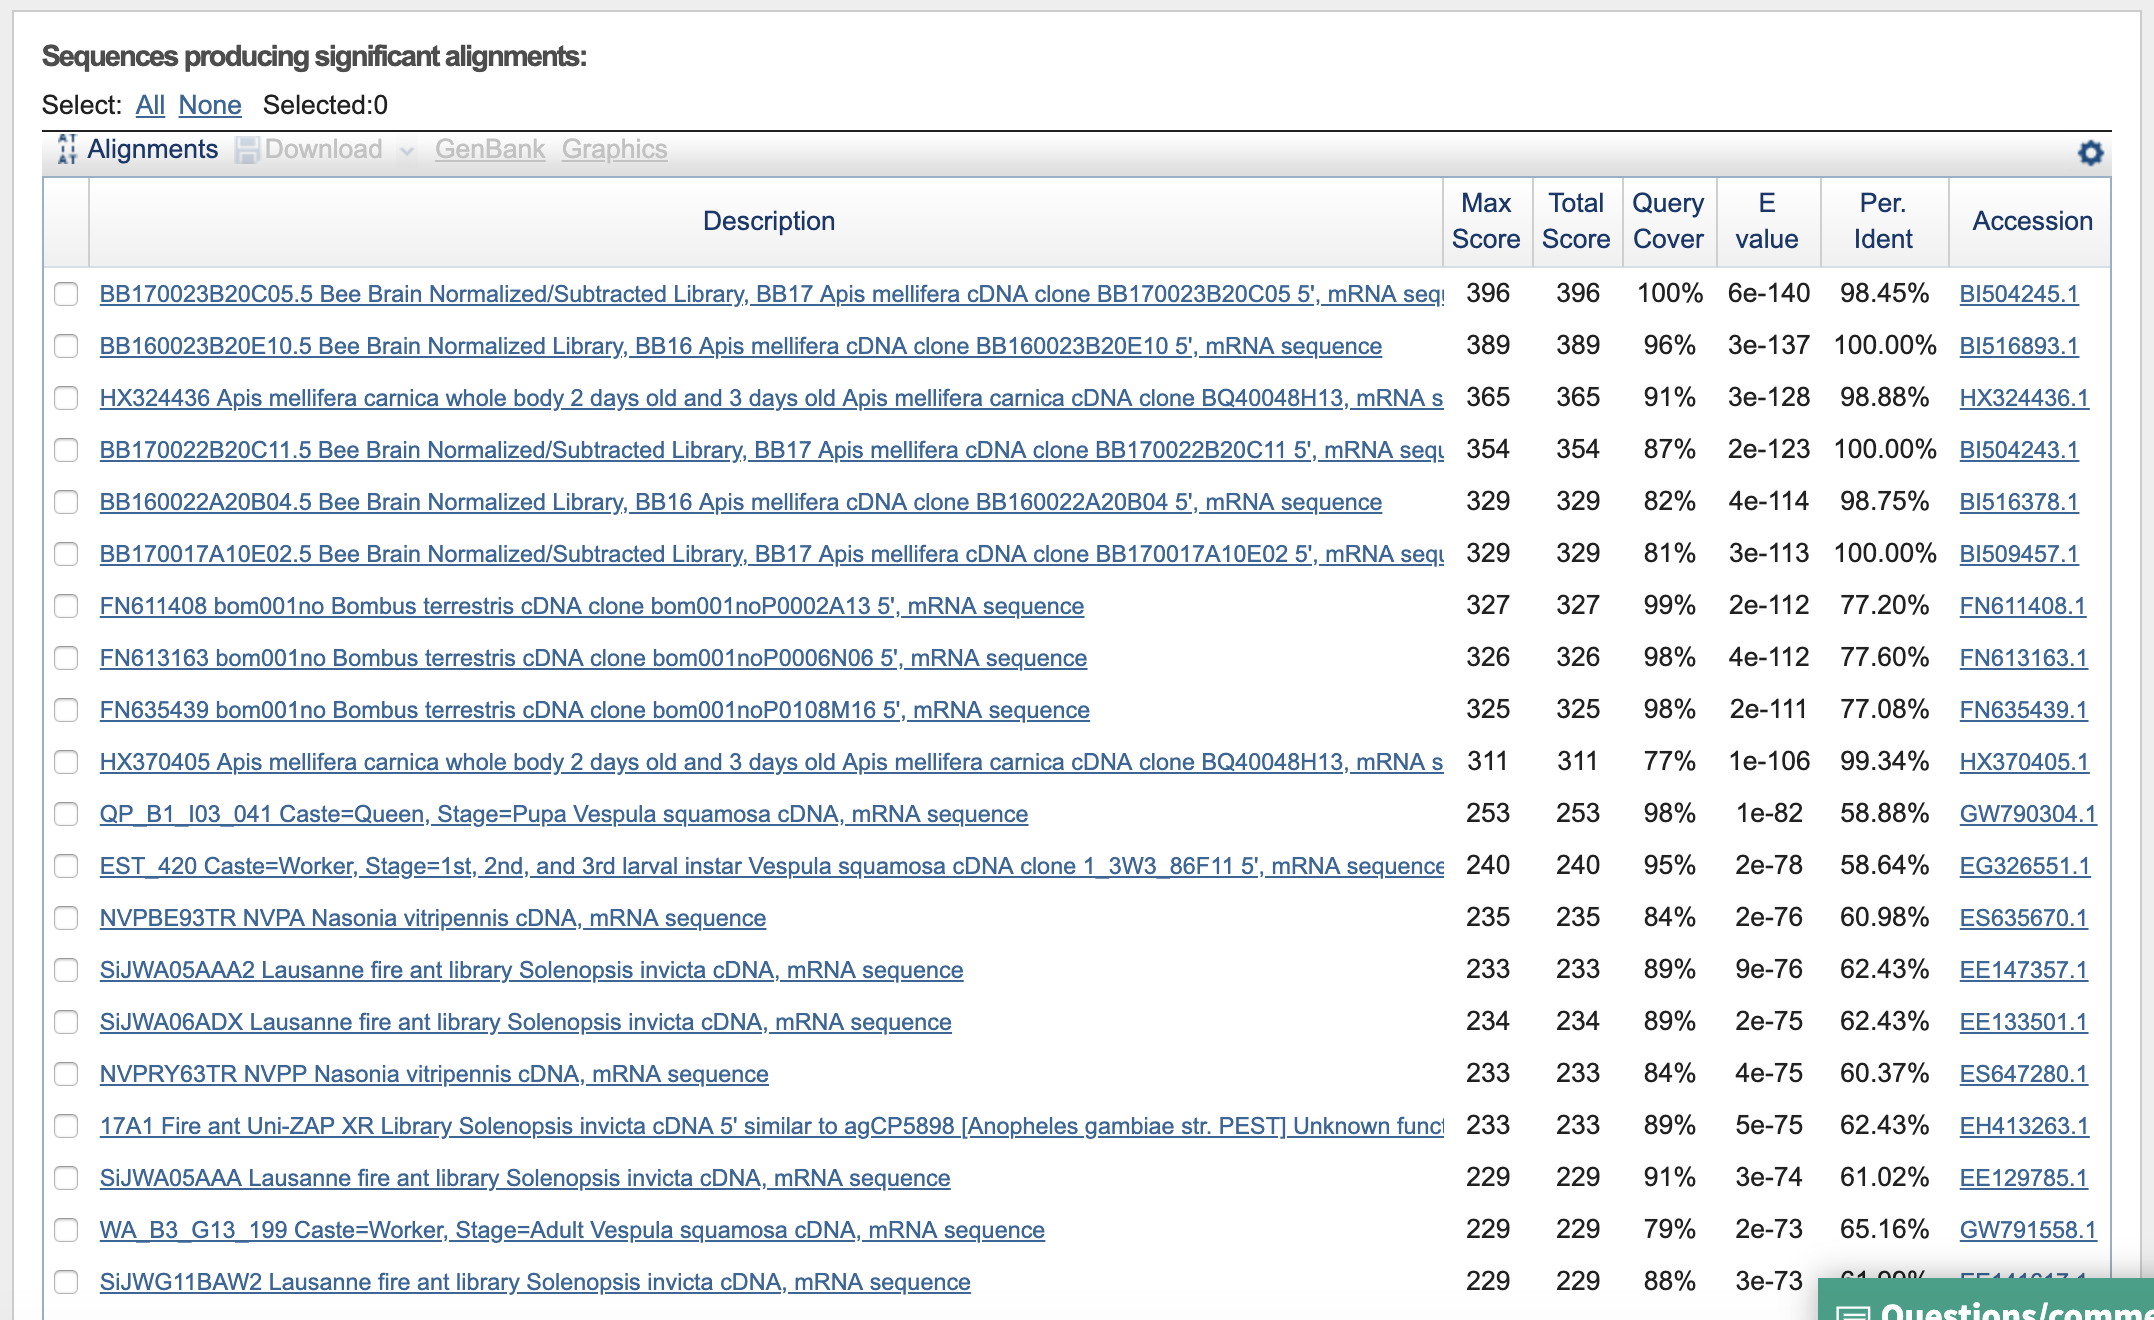
\includegraphics{q2a.png}

Some select hits of interest: 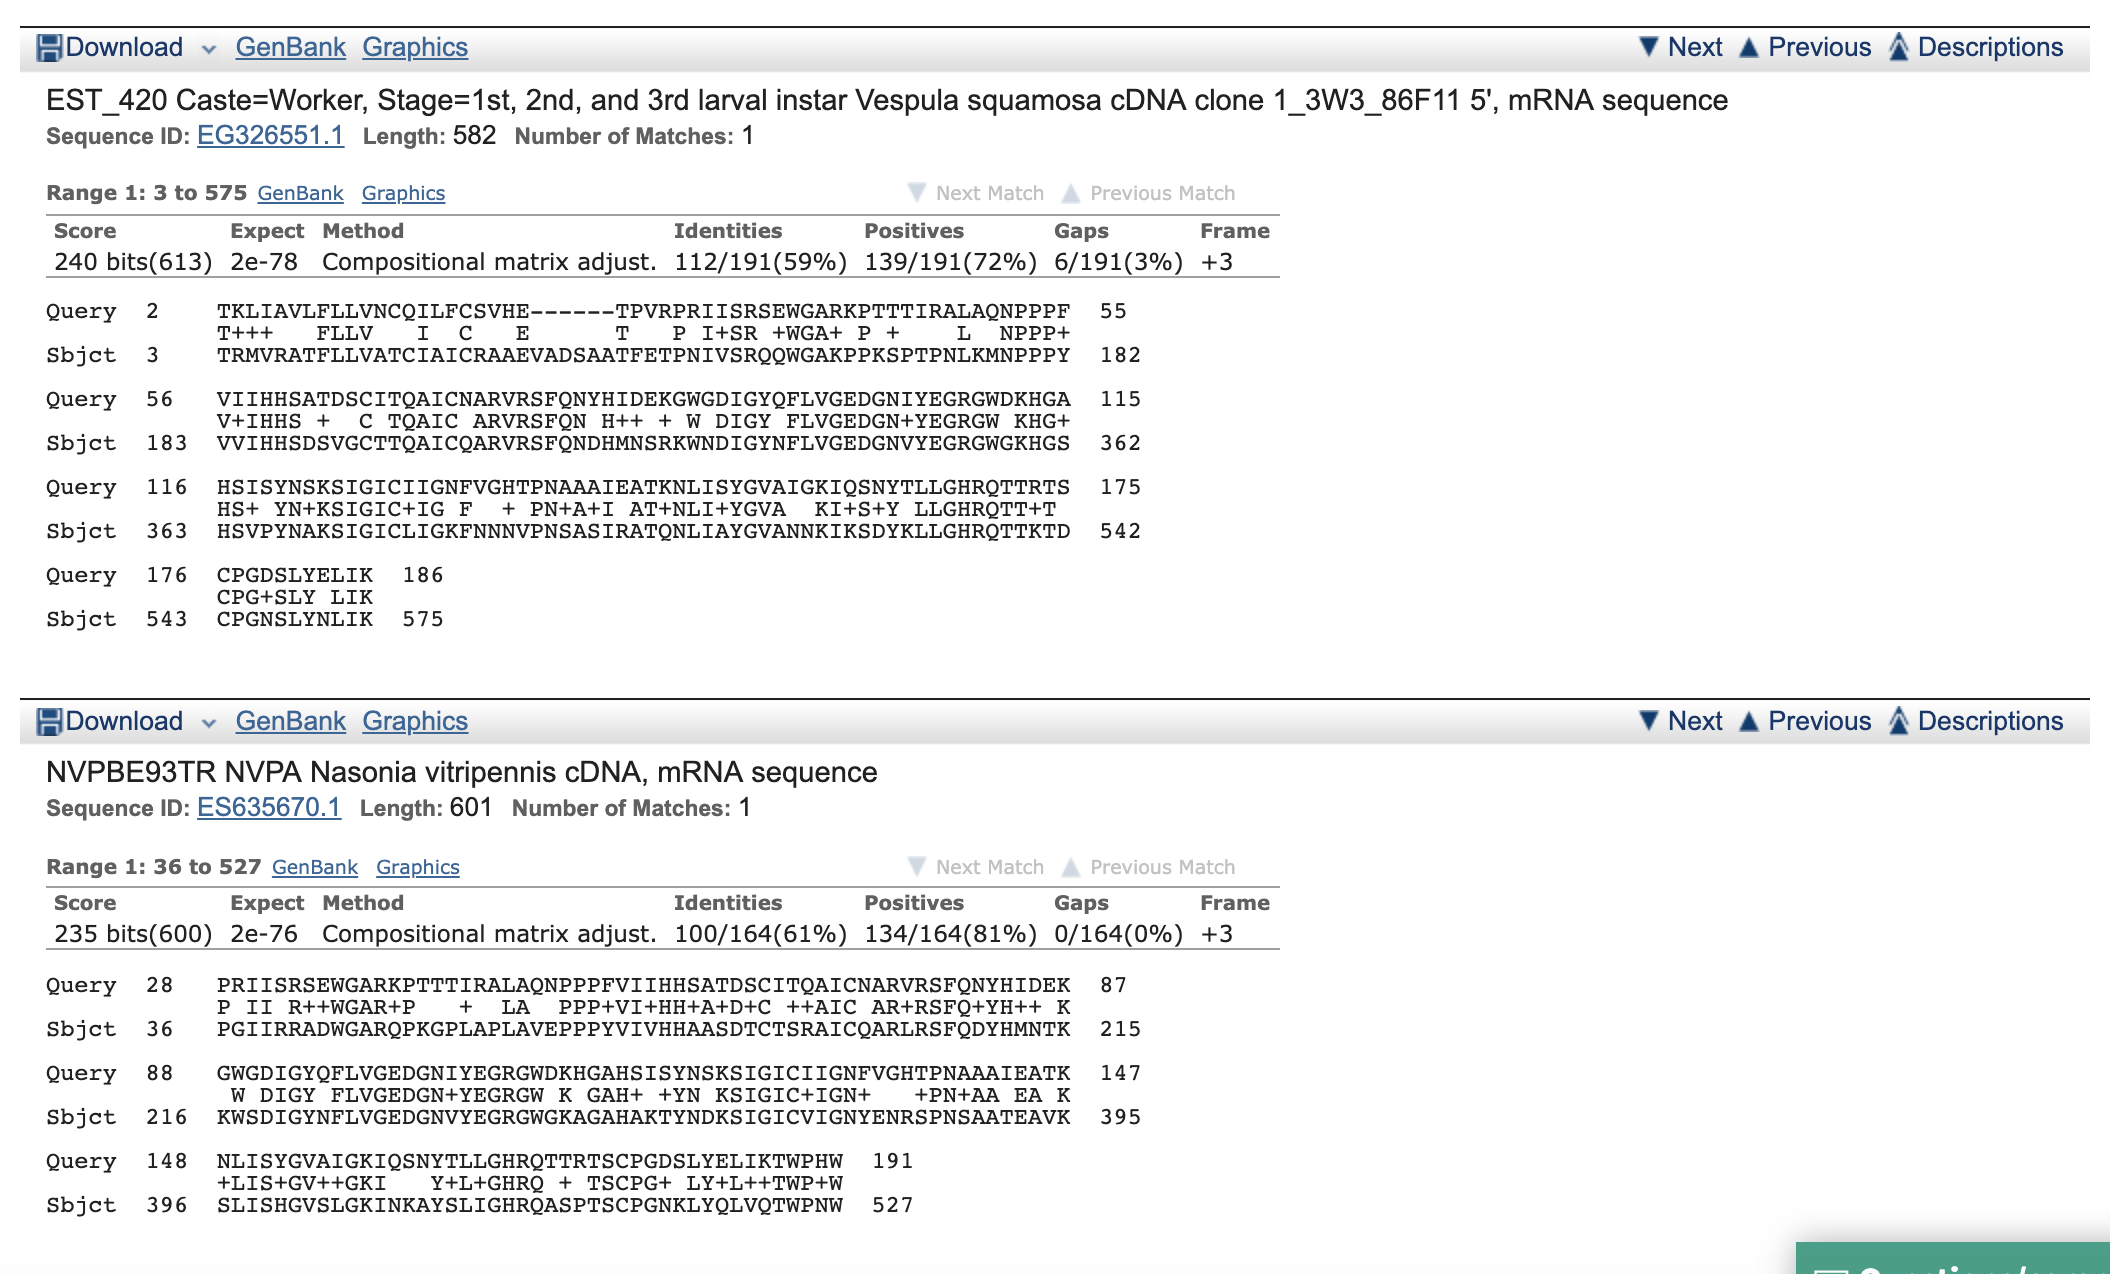
\includegraphics{q2b.png} On the BLAST
results, clearly indicate a match that represents a protein sequence,
encoded from some DNA sequence, that is homologous to your query
protein. I need to be able to inspect the pairwise alignment you have
selected, including the E value and score. It should be labeled a
``genomic clone'' or ``mRNA sequence'', etc. - but include no functional
annotation.

I am interested in FN611408.1 (\emph{Bombus terrestris)}; GW790304.1,
(\emph{Vespula squamosa}); EE147357.1 (\emph{Solenopsis invicta}),
ES647280.1 (\emph{Nasonia vitripens}) etc.

All of these sequences appear to be hitherto unannotated mRNAs, all of
which belong to Hymenopterans. Vespula squamosa is likely the most
under-annotated, as it is not a model organism or
agriculturally-relevant species.

\section{Question 3}\label{question-3}

\begin{quote}
Gather information about this ``novel'' protein. At a minimum, show me
the protein sequence of the ``novel'' protein as displayed in your BLAST
results from {[}Q2{]} as FASTA format (you can copy and paste the
aligned sequence subject lines from your BLAST result page if necessary)
or translate your novel DNA sequence using a tool called EMBOSS Transeq
at the EBI. Don't forget to translate all six reading frames; the ORF
(open reading frame) is likely to be the longest sequence without a stop
codon. It may not start with a methionine if you don't have the complete
coding region. Make sure the sequence you provide includes a
header/subject line and is in traditional FASTA format. Here, tell me
the name of the novel protein, and the species from which it derives. It
is very unlikely (but still definitely possible) that you will find a
novel gene from an organism such as S. cerevisiae, human or mouse,
because those genomes have already been thoroughly annotated. It is more
likely that you will discover a new gene in a genome that is currently
being sequenced, such as bacteria or plants or protozoa.
\end{quote}

\subsubsection{The Target Sequence}\label{the-target-sequence}

Below follows the FASTA sequence for the cDNA clone from \emph{V.
squamosa}: GW790304.1 QP\_B1\_I03\_041 Caste=Queen, Stage=Pupa Vespula
squamosa cDNA, mRNA sequence
CGAGAATGGTACGAGCAACGTTTCTACTTGTTGCAACGTGCATTGCAATTTGCCGTGCAGCGGAAGTTGCAGATTCGGCT
GCAACCTTTGAAACACCTAATATCGTTTCAAGACAACAATGGGGAGCTAAACCGCCGAAAAGCCCTACGCCTAATCTTAA
AATGAATCCACCTCCTTACGTTGTTATTCATCATTCGGATTCAGTTGGTTGTACCACTCAAGCAATTTGTCAGGCTAGAG
TTAGAAGTTTTCAGAATGATCATATGAACTCGAGAAAATGGAATGACATCGGCTACAACTTTTTGGTCGGTGAAGATGGT
AATGTTTACGAAGGTCGTGGCTGGGGTAAACATGGCTCCCATTCAGTCCCGTACAATGCCAAGAGTATCGGTATTTGCCT
TATTGGTAAATTTAACAATAACGTACCGAATTCAGCGAGTATTCGAGCAACACAAAATTTGATAGCTTACGGAGTAGCTA
ACAACAAAATCAAATCCGATTATAAGCTTCTTGGCCATCGACAAACCACTAAAACTGATTGTCCTGGAAATTCTCTATAC
AATTTGATTAAAACATGGCCTCACTGGACCGACACGCCATAAGAAATATAATCGTTATGCGATTAAATTAATCTACCAAG
TATAACGTCTTATTGTTTTGGACTCGACGATCATTGGAAATTAACGATCATCGGATCGATAACTTTTGTTGACTTTTCTT
TAATTAACGATGGATACCTTCAAATTCGATTTTCGTGCGAACATTTTTACTTGATGTTTCGTAAAGGAAGAG

BLAST gives this translated protein sequence: 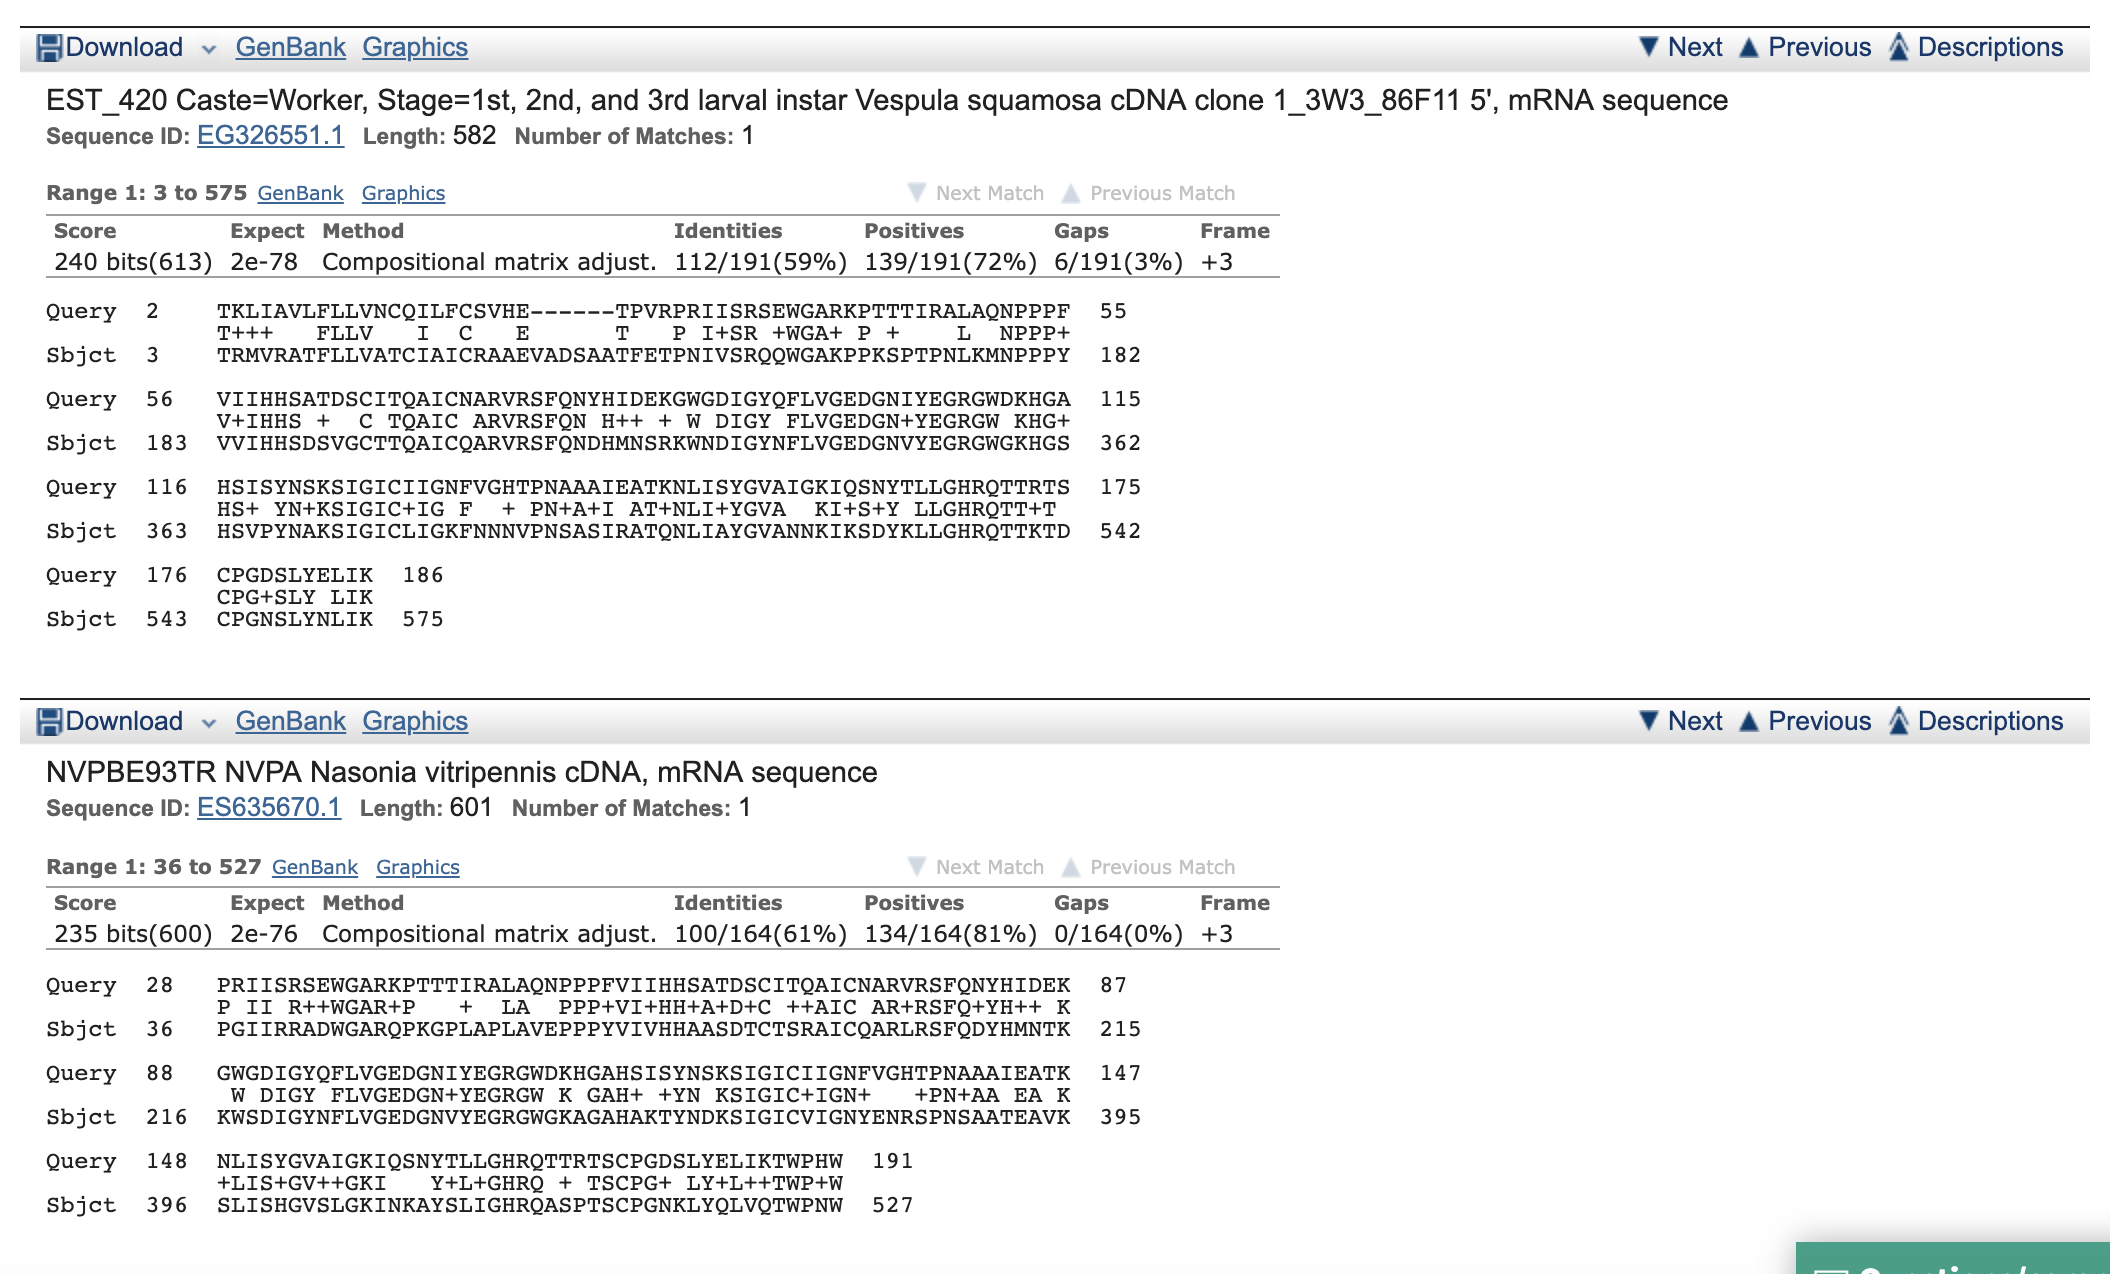
\includegraphics{q3.png}

\subsubsection{EMBOSS protein
translation}\label{emboss-protein-translation}

I put this sequence through EMBOSS Transeq (EBI) for the following
translations (please note, to avoid confusion with RMD, I have
substituted the ``*" code for stop codons with ``x''): GW790304.1\_1
QP\_B1\_I03\_041 Caste=Queen, Stage=Pupa Vespula squamosa cDNA, mRNA
sequence REWYEQRFYLLQRALQFAVQRKLQIRLQPLKHLISFQDNNGELNRRKALRLILKxIHLLT
LLFIIRIQLVVPLKQFVRLELEVFRMIIxTRENGMTSATTFWSVKMVMFTKVVAGVNMAP
IQSRTMPRVSVFALLVNLTITYRIQRVFEQHKIxxLTExLTTKSNPIISFLAIDKPLKLI
VLEILYTIxLKHGLTGPTRHKKYNRYAIKLIYQVxRLIVLDSTIIGNxRSSDRxLLLTFL
xLTMDTFKFDFRANIFTxCFVKEE

GW790304.1\_2 QP\_B1\_I03\_041 Caste=Queen, Stage=Pupa Vespula squamosa
cDNA, mRNA sequence
ENGTSNVSTCCNVHCNLPCSGSCRFGCNLxNTxYRFKTTMGSxTAEKPYAxSxNESTSLR
CYSSFGFSWLYHSSNLSGxSxKFSExSYELEKMExHRLQLFGRxRWxCLRRSWLGxTWLP
FSPVQCQEYRYLPYWxIxQxRTEFSEYSSNTKFDSLRSSxQQNQIRLxASWPSTNHxNxL
SWKFSIQFDxNMASLDRHAIRNIIVMRLNxSTKYNVLLFWTRRSLEINDHRIDNFCxLFF
NxRWIPSNSIFVRTFLLDVSxRKX

\textbf{GW790304.1\_3 QP\_B1\_I03\_041 Caste=Queen, Stage=Pupa Vespula
squamosa cDNA, mRNA sequence}
RMVRATFLLVATCIAICRAAEVADSAATFETPNIVSRQQWGAKPPKSPTPNLKMNPPPYV
VIHHSDSVGCTTQAICQARVRSFQNDHMNSRKWNDIGYNFLVGEDGNVYEGRGWGKHGSH
SVPYNAKSIGICLIGKFNNNVPNSASIRATQNLIAYGVANNKIKSDYKLLGHRQTTKTDC
PGNSLYNLIKTWPHWTDTPxEIxSLCDxINLPSITSYCFGLDDHWKLTIIGSITFVDFSL
INDGYLQIRFSCEHFYLMFRKGRX

(This appears to be the best option to go with; longest ORF.)

GW790304.1\_4 QP\_B1\_I03\_041 Caste=Queen, Stage=Pupa Vespula squamosa
cDNA, mRNA sequence
LFLYETSSKNVRTKIEFEGIHRxLKKSQQKLSIRxSLISNDRRVQNNKTLYLVDxFNRIT
IIFLMACRSSEAMFxSNCIENFQDNQFxWFVDGQEAYNRIxFCCxLLRKLSNFVLLEYSL
NSVRYCxIYQxGKYRYSWHCTGLNGSHVYPSHDLRKHYHLHRPKSCSRCHSIFSSSYDHS
ENFxLxPDKLLEWYNQLNPNDExQRKEVDSFxDxAxGFSAVxLPIVVLKRYxVFQRLQPN
LQLPLHGKLQCTLQQVETLLVPFS

GW790304.1\_5 QP\_B1\_I03\_041 Caste=Queen, Stage=Pupa Vespula squamosa
cDNA, mRNA sequence
LPLRNIKxKCSHENRIxRYPSLIKEKSTKVIDPMIVNFQxSSSPKQxDVILGRLIxSHND
YISYGVSVQxGHVLIKLYREFPGQSVLVVCRWPRSLxSDLILLLATPxAIKFCVARILAE
FGTLLLNLPIRQIPILLALYGTEWEPCLPQPRPSxTLPSSPTKKLxPMSFHFLEFIxSFx
KLLTLAxQIAxVVQPTESExxITTxGGGFILRLGVGLFGGLAPHCCLETILGVSKVAAES
ATSAARQIAMHVATSRNVARTILX

GW790304.1\_6 QP\_B1\_I03\_041 Caste=Queen, Stage=Pupa Vespula squamosa
cDNA, mRNA sequence
SSFTKHQVKMFARKSNLKVSIVNxRKVNKSYRSDDRxFPMIVESKTIRRYTWxINLIAxR
LYFLWRVGPVRPCFNQIVxRISRTISFSGLSMAKKLIIGFDFVVSYSVSYQILCCSNTRx
IRYVIVKFTNKANTDTLGIVRDxMGAMFTPATTFVNITIFTDQKVVADVIPFSRVHMIIL
KTSNSSLTNCLSGTTNxIRMMNNNVRRWIHFKIRRRAFRRFSSPLLSxNDIRCFKGCSRI
CNFRCTANCNARCNKxKRCSYHSR

\subsection{Question 4}\label{question-4}

\begin{quote}
Prove that this gene, and its corresponding protein, are novel. For the
purposes of this project, ``novel'' is defined as follows. Take the
protein sequence (your answer to {[}Q3{]}), and use it as a query in a
blastp search of the nr database at NCBI. * If there is a match with
100\% amino acid identity to a protein in the database, from the same
species, then your protein is NOT novel (even if the match is to a
protein with a name such as ``unknown''). Someone has already found and
annotated this sequence, and assigned it an accession number. * If the
top match reported has less than 100\% identity, then it is likely that
your protein is novel, and you have succeeded. * If there is a match
with 100\% identity, but to a different species than the one you started
with, then you have likely succeeded in finding a novel gene. * If there
are no database matches to the original query from {[}Q1{]}, this
indicates that you have partially succeeded: yes, you may have found a
new gene, but not is not actually homologous to the original query. You
should probably start over.
\end{quote}

The BLASTp results from the selected sequence above follow below:
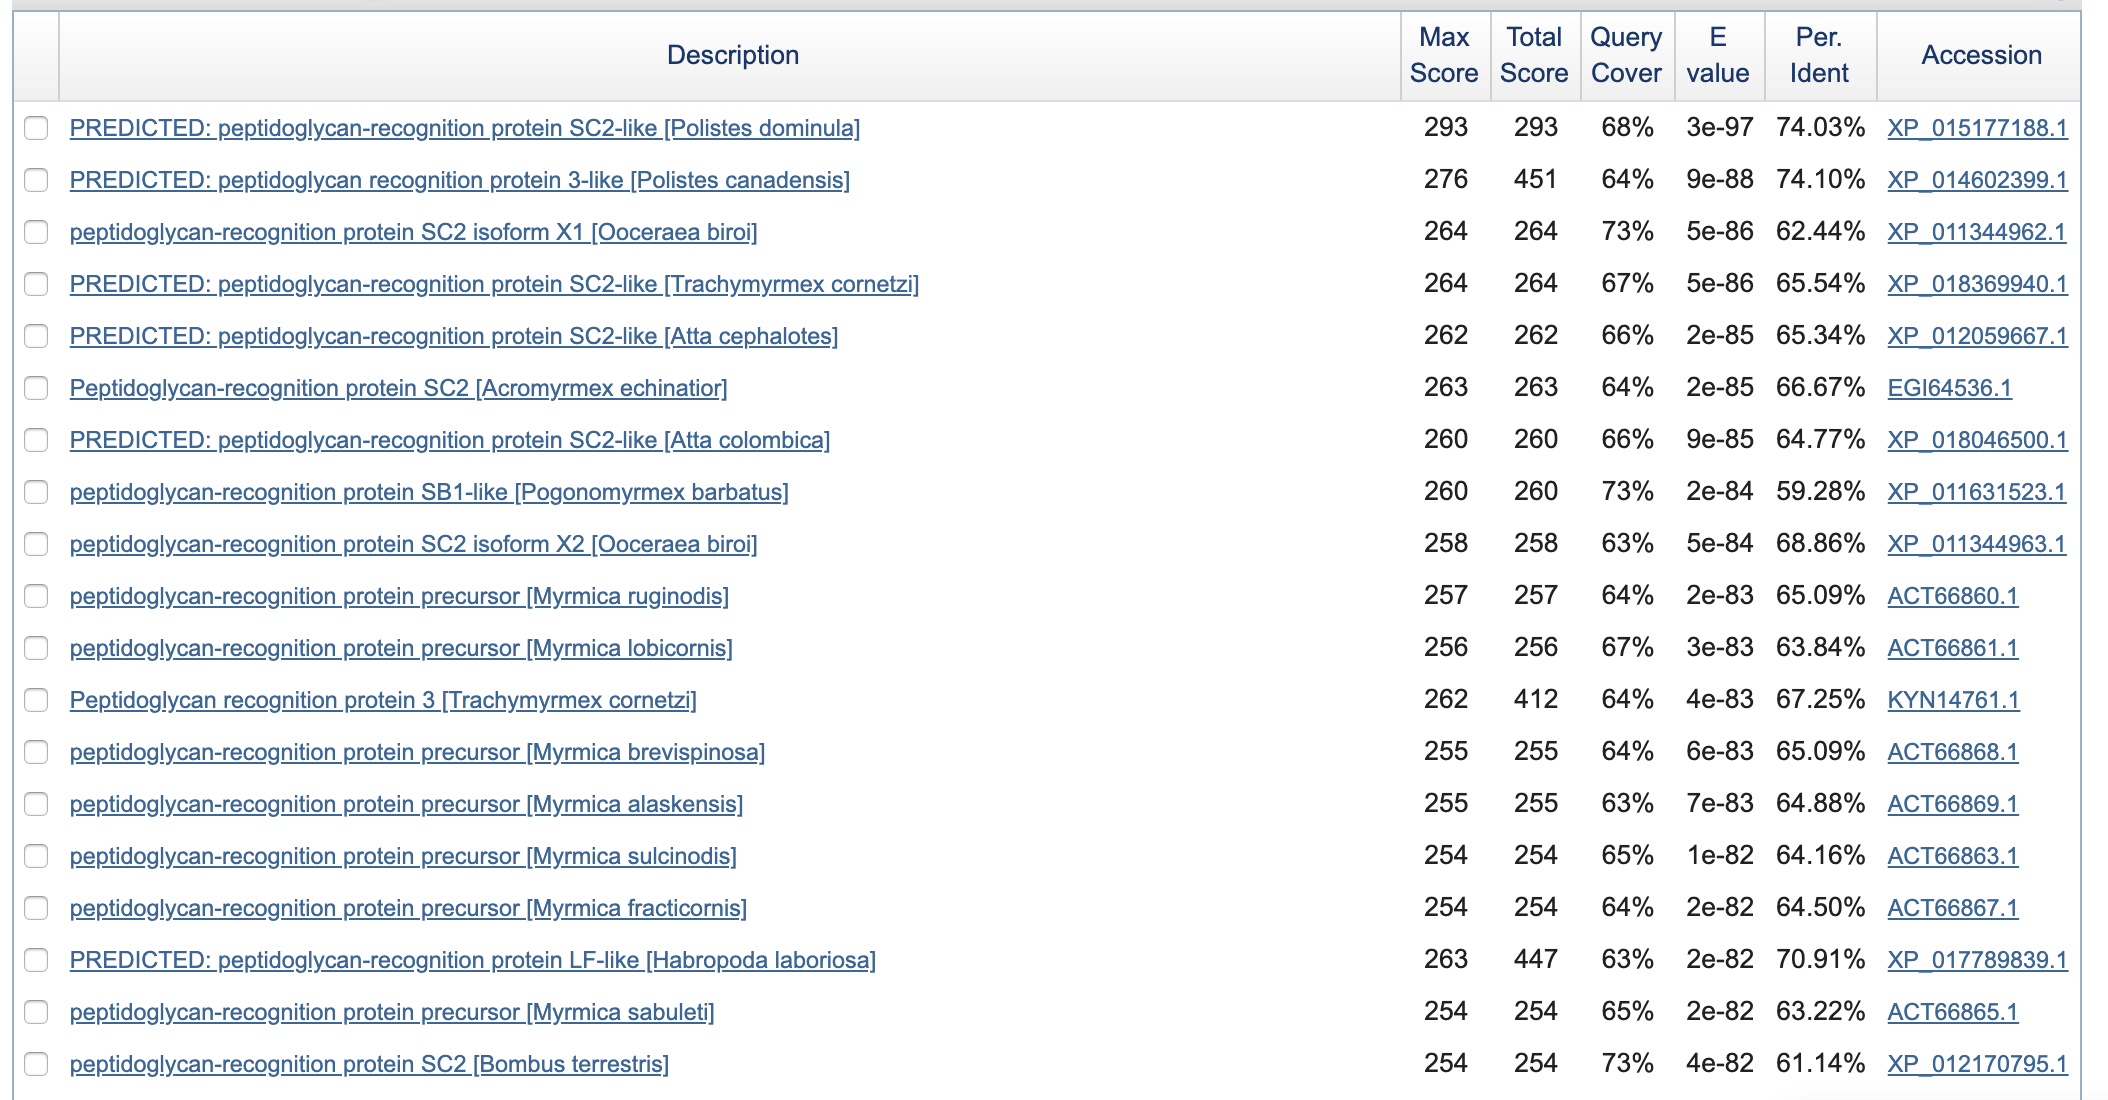
\includegraphics{q4.png} The top hits are not exact matches, but appear
to be related to the function from the original \emph{A. mellifera}
gene, as well as other closely related species, suggesting there is
homology among these sequences, and potentially similar function in this
\emph{V. squamosa} sequence.

\section{Question 5}\label{question-5}

\begin{quote}
Generate a multiple sequence alignment with your novel protein, your
original query protein, and a group of other members of this family from
different species. A typical number of proteins to use in a multiple
sequence alignment for this assignment purpose is a minimum of 5 and a
maximum of 20 - although the exact number is up to you. Include the
multiple sequence alignment in your report. Use Courier font with a size
appropriate to fit page width.
\end{quote}

\subsubsection{Input Sequences}\label{input-sequences}

List of sequences used for multiple alignment using MUSCLE (EBI); the
first if the original Apis mellifera reference sequence, the second is
the presumed Vespula squamosa sequence, and the other 9 are sequences
from other Hymenoptera.

\begin{itemize}
\tightlist
\item
  NP\_001157188.1 peptidoglycan-recognition protein S2 precursor {[}Apis
  mellifera{]}
  MTKLIAVLFLLVNCQILFCSVHETPVRPRIISRSEWGARKPTTTIRALAQNPPPFVIIHHSATDSCITQA
  ICNARVRSFQNYHIDEKGWGDIGYQFLVGEDGNIYEGRGWDKHGAHSISYNSKSIGICIIGNFVGHTPNA
  AAIEATKNLISYGVAIGKIQSNYTLLGHRQTTRTSCPGDSLYELIKTWPHWSSI
\item
  GW790304.1\_3 QP\_B1\_I03\_041 Caste=Queen, Stage=Pupa Vespula
  squamosa cDNA, mRNA sequence
  RMVRATFLLVATCIAICRAAEVADSAATFETPNIVSRQQWGAKPPKSPTPNLKMNPPPYV
  VIHHSDSVGCTTQAICQARVRSFQNDHMNSRKWNDIGYNFLVGEDGNVYEGRGWGKHGSH
  SVPYNAKSIGICLIGKFNNNVPNSASIRATQNLIAYGVANNKIKSDYKLLGHRQTTKTDC
  PGNSLYNLIKTWPHWTDTPxEIxSLCDxINLPSITSYCFGLDDHWKLTIIGSITFVDFSL
  INDGYLQIRFSCEHFYLMFRKGRx
\item
  XP\_011344962.1 peptidoglycan-recognition protein SC2 isoform X1
  {[}Ooceraea biroi{]}
  MYIARRTTVLIFAAVYVTLVAQEAAARPNTGGQIIPNIISRAQWGAKSPKSPLSNLAKKPAPYVIIHHST
  DTGCETQALCQAKVRGFQNYHMNSKGWTDIGYNFLVGEDGNVYEGRGWGKKGSHSKPFNGKSIGICIIGD
  YSNRTPKPAAVQAVSKLIAYGVSNDEIKSDYILLGHRQTGQTTCPGNSLYGMIKSWPHWQSSA
\item
  XP\_011631523.1 peptidoglycan-recognition protein SB1-like
  {[}Pogonomyrmex barbatus{]}
  MYITKRTTLIFATVYVTLIVQETVATSPNIISRSEWGARAPKSRAPNLKLKPAPYVLIHHSTGSGCETQA
  LCQLKVRQFQNEHMNTKGWSDIGYNFLVGEDGNVYEGRGWGKQGAHSIPFNKKSIGICIIGDYRKRTPNA
  MAVQAVANLIAQGVQNGEIKSDYKLLGHRQTWPTICPGDSLYTMIKSWPHWSERE
\item
  XP\_012170795.1 peptidoglycan-recognition protein SC2 {[}Bombus
  terrestris{]}
  MTKLIAVILLLASCQVLFCAVHKTPVRPSIISRSEWGANAPKSTLRNLAEEPAPFVIIHHSASDSCTTRA
  ICQARVRSFQNHHMNQKGWNDIGYNFLVGEDGNIYEGRGWGKHGAHSTPYNSKSIGICMIGNFVGHNPSA
  AAIKAVKDLIEYGVTLGKIQENYTLLGHRQTTSTSCPGDSLYQLIQTWPHWSSI
\item
  XP\_011143830.1 peptidoglycan-recognition protein SC2 isoform X1
  {[}Harpegnathos saltator{]}
  MFVATSTSAVFIAAAYLTLLIPETAATAPTIISRAQWGARAPKHQAANLARKPAPYVVLHHSTGNGCVTQ
  AICQLKVREFQNYHMNSKKWSDVGYNFIVGEDGNIYEGRGWGKQGAHSKPFNNKSIGICIIGDYTNRTPN
  SAAVQAVDSLIAYGVSSGEIKNDYKLLGHRQTWQTNCPGNSLYTMMQSWPHWAAAA
\item
  XP\_014205259.1 peptidoglycan-recognition protein SC2-like
  {[}Copidosoma floridanum{]}
  MGKRVLLFVLMLMVKQGEFWSTKTFENPKFTIITRSEWGAQPPKGNVGSLKTLPATYVVIHHAASLSCTN
  RAICQARIRTIQNFHMKTEKLQDIGFNFLVGEDGNVYEGRGWEKAGAHAENFNDKSIGICVIGNFDKTSP
  SHATLAAIKNLISHGVSQGKLNSQYILIGHRQAETLSCPGHYLYQLIQTWSHWRKISQNAA
\item
  XP\_017886197.1 peptidoglycan-recognition protein SB1-like {[}Ceratina
  calcarata{]}
  MPVFKLVVAFNYLLLIVPTYSLNTVEIVPNIISRQNWHARQPVERELLEVTPTPYVVIHHGGEPKYCYDE
  KTCSAIVRQYQNFHIDDRHWFDIGYSFVIGEDGNVYEGRGWDYVGAHAPGYNTQSIGICIIGDFSNFVPN
  EKALKTLNDLIKYGVKLRKIRGDYHILGHRQARSTLCPGTAFYKYVQTLPRWTNHPIPNYSNGTTTTLAL
\item
  XP\_028138990.1 peptidoglycan-recognition protein 2-like {[}Diabrotica
  virgifera virgifera{]}
  MIYSRYLWIVCVVLSLFYQTNCECPKIYTRNEWSARKALSTRPLREDPPPYVVVHHSATRSCFSVEDCSK
  LVKSIQDYHIDHNGWDDIGYNFLIGGDGTIYEGRGYGLHGAHSIPYNARSLGVCLLGSFKDTNPPNVQLK
  ALEDFLSCAAADHKIIADYHLIGHRQADKTECPGDRVHAVIEKWPHFEANPQDASPKKL
\item
  NP\_001037560.1 peptidoglycan recognition protein S2 precursor
  {[}Bombyx mori{]}
  MLVAPSLLLLVFLVSFGTLNAASECGEIPITEWSGTESRRKQPLKSPIDLVVIQHTVSNDCFTDEECLLS
  VNSLRQHHMRLAGFKDLGYSFVAGGNGKIYEGAGWNHIGAHTLHYNNISIGIGFIGDFREKLPTQQALQA
  VQDFLACGVENNLLTEDYHVVGHQQLINTLSPGAVLQSEIESWPHWLDNARKVLG
\item
  ALN97023.1 peptidoglycan recognition protein S2 {[}Microplitis
  mediator{]}
  MFYVIEVILLNALFAFAAGQSTVNIISRQEWGARLPKEPPINLTINPPAFIVIHHSGRGAGCTTQALCQA
  KVRSFQDFHMDFREWDDIGYNYLIGEDGNVYEGRGWGIKGAHFPAYNARSLGLCFIGNFDKKIPAPAAIK
  TAKNFLDYAVTLGKLQSNYTLIGHRQGRSTTCPGDKLFELIQSWPKWKNVTTD
\end{itemize}

\subsubsection{MUSCLE Output}\label{muscle-output}

I ran the MUSCLE with default parameters to produce the following
ClustalW output: CLUSTAL multiple sequence alignment by MUSCLE (3.8).

\begin{figure}
\centering
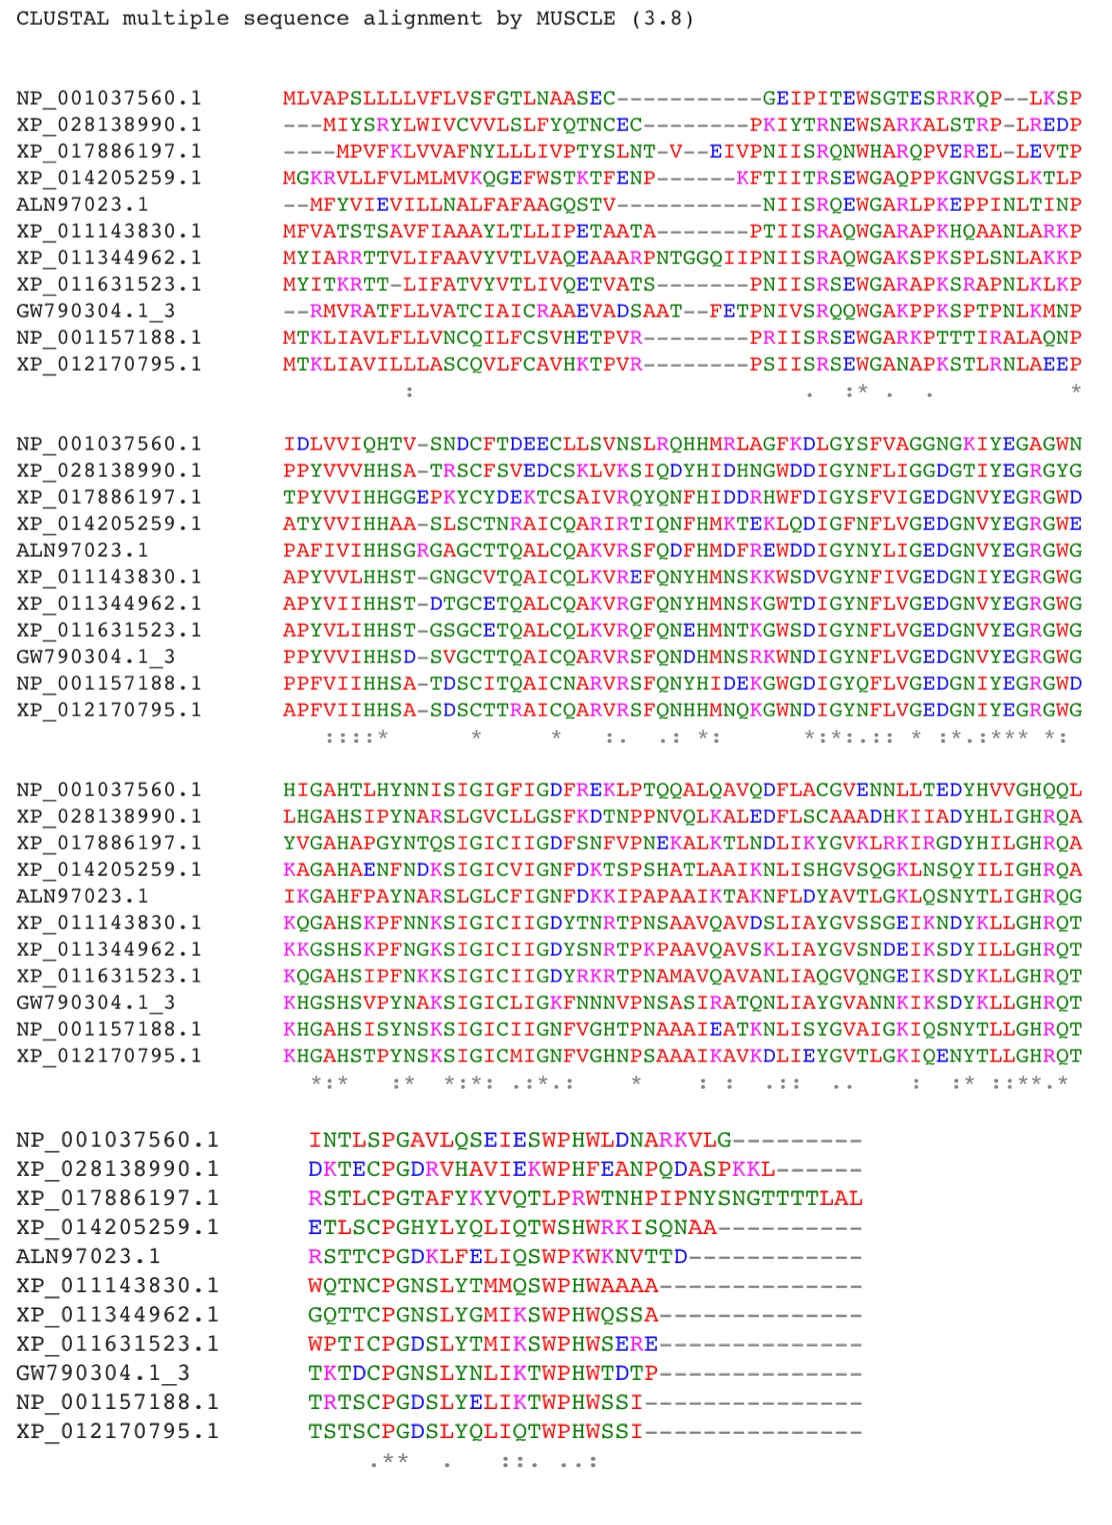
\includegraphics{q5.png}
\caption{q5}
\end{figure}

\section{Question 6}\label{question-6}

Create a phylogenetic tree, using either a parsimony or distance-based
approach. Bootstrapping and tree rooting are optional. Use ``simple
phylogeny'' online from the EBI or any respected phylogeny program (such
as MEGA, PAUP, or Phylip). Paste an image of your Cladogram or tree
output in your report.

I ported the output from the previous question to Simple Phylogeny (EBI)
and asked it to make me a cladogram using default parameters.

\begin{figure}
\centering
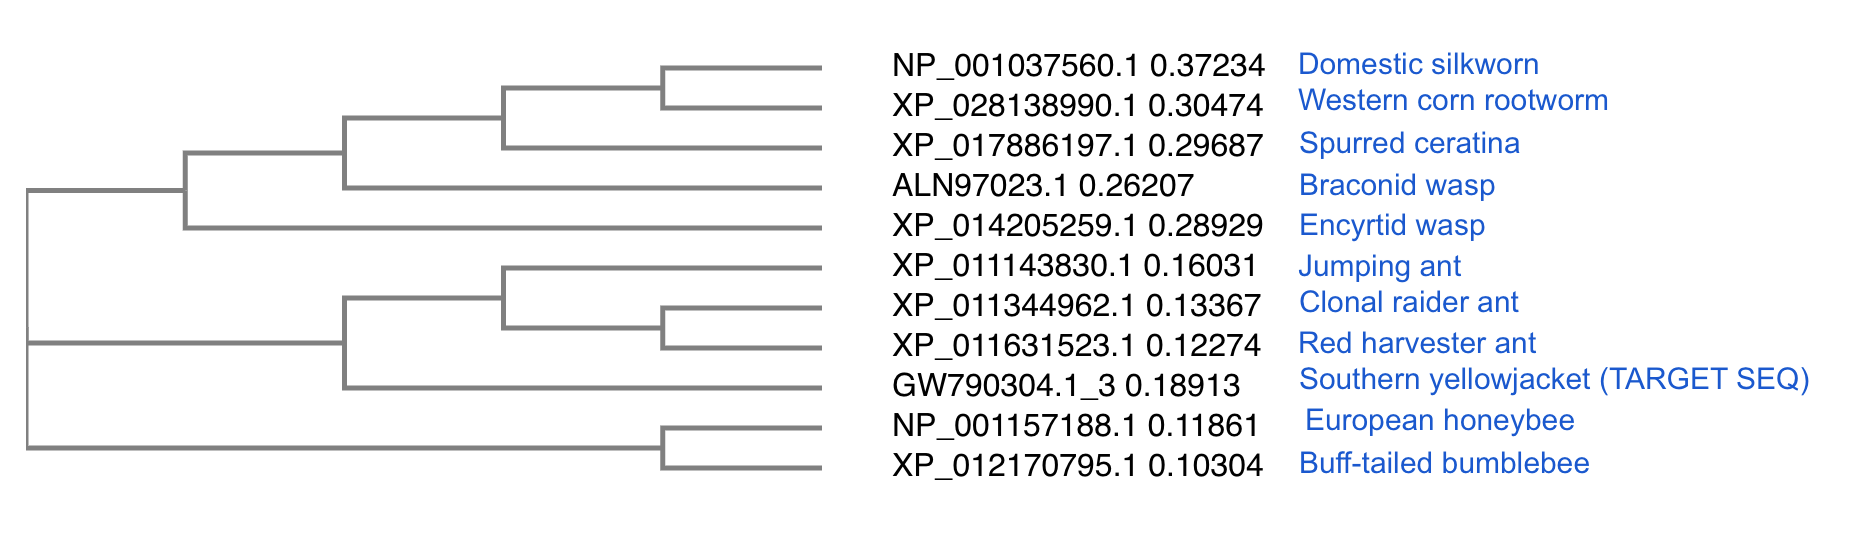
\includegraphics{q6_BGGN213_FindAGene_Q6_Cladogram.png}
\caption{q6}
\end{figure}

Below is a key describing each branch in order:

\begin{longtable}[]{@{}llll@{}}
\toprule
Accession & Scientific name & Common name & General
Detail\tabularnewline
\midrule
\endhead
NP\_001037560.1 & {[}B. mori{]} & Domestic silkworm &
(Moth)\tabularnewline
XP\_028138990.1 & {[}D. virgifera virgifera{]} & Western corn rootworm &
(Beetle)\tabularnewline
XP\_017886197.1 & {[}C. calcarata{]} & Spurred ceratina & (Apid
bee)\tabularnewline
ALN97023.1 & {[}M. mediator{]} & NCN & (Braconid wasp)\tabularnewline
XP\_014205259.1 & {[}C. floridanum{]} & NCN & (Encyrtid
wasp)\tabularnewline
XP\_011143830.1 & {[}H. saltator{]} & Jumping ant & (Ant)\tabularnewline
XP\_011344962.1 & {[}O. biroi{]} & Clonal raider ant &
(Ant)\tabularnewline
XP\_011631523.1 & {[}P. barbatus{]} & Red harvester ant &
(Ant)\tabularnewline
GW790304.1\_3 & {[}V. squamosa, Target{]} & Southern yellowjacket &
(Vespid wasp)\tabularnewline
NP\_001157188.1 & {[}A. mellifera{]} & European honeybee & (Apid
bee)\tabularnewline
XP\_012170795.1 & {[}B. terrestris{]} & Buff-tailed bumblebee & (Apid
bee)\tabularnewline
\bottomrule
\end{longtable}

As an interesting note, we see that the largely solitary hymenoptera
(the Ceratina and parasitic wasps) cluster with the outgroup moth and
beetle, whereas the highly social lineages (the ants, bumblebees,
yellowjackets and honey bees) cluster together. It's not particularly
relevant for this project, but it's cool to know that this supports the
current hypothesis that social living deeply affects immune response in
Hymenoptera, notably a reduction in function of individual immunes genes
in favor of social behaviors that support group immunity.

\section{Question 7}\label{question-7}

For Question 7, we will make a heatmap of the alignment we ran of the V.
squamosa predicted PGRP S2 with the base sequence from A. mellifera, and
the 9 other PRGP-associated sequences.

\subsubsection{Making the alignment in
R}\label{making-the-alignment-in-r}

\begin{Shaded}
\begin{Highlighting}[]
\NormalTok{pgrp <-}\StringTok{ }\KeywordTok{read.fasta}\NormalTok{(}\StringTok{"aln-fasta.txt"}\NormalTok{) }\CommentTok{# This file contains aligned sequences}
\KeywordTok{head}\NormalTok{(pgrp)}
\end{Highlighting}
\end{Shaded}

\begin{verbatim}
## $id
##  [1] "NP_001037560.1" "XP_028138990.1" "XP_017886197.1" "XP_014205259.1"
##  [5] "ALN97023.1"     "XP_011143830.1" "XP_011344962.1" "XP_011631523.1"
##  [9] "GW790304.1_3"   "NP_001157188.1" "XP_012170795.1"
## 
## $ali
##                [,1] [,2] [,3] [,4] [,5] [,6] [,7] [,8] [,9] [,10] [,11]
## NP_001037560.1 "M"  "L"  "V"  "A"  "P"  "S"  "L"  "L"  "L"  "L"   "V"  
## XP_028138990.1 "-"  "-"  "-"  "M"  "I"  "Y"  "S"  "R"  "Y"  "L"   "W"  
## XP_017886197.1 "-"  "-"  "-"  "-"  "M"  "P"  "V"  "F"  "K"  "L"   "V"  
## XP_014205259.1 "M"  "G"  "K"  "R"  "V"  "L"  "L"  "F"  "V"  "L"   "M"  
## ALN97023.1     "-"  "-"  "M"  "F"  "Y"  "V"  "I"  "E"  "V"  "I"   "L"  
## XP_011143830.1 "M"  "F"  "V"  "A"  "T"  "S"  "T"  "S"  "A"  "V"   "F"  
## XP_011344962.1 "M"  "Y"  "I"  "A"  "R"  "R"  "T"  "T"  "V"  "L"   "I"  
## XP_011631523.1 "M"  "Y"  "I"  "T"  "K"  "R"  "T"  "T"  "-"  "L"   "I"  
## GW790304.1_3   "-"  "-"  "R"  "M"  "V"  "R"  "A"  "T"  "F"  "L"   "L"  
## NP_001157188.1 "M"  "T"  "K"  "L"  "I"  "A"  "V"  "L"  "F"  "L"   "L"  
## XP_012170795.1 "M"  "T"  "K"  "L"  "I"  "A"  "V"  "I"  "L"  "L"   "L"  
##                [,12] [,13] [,14] [,15] [,16] [,17] [,18] [,19] [,20] [,21]
## NP_001037560.1 "F"   "L"   "V"   "S"   "F"   "G"   "T"   "L"   "N"   "A"  
## XP_028138990.1 "I"   "V"   "C"   "V"   "V"   "L"   "S"   "L"   "F"   "Y"  
## XP_017886197.1 "V"   "A"   "F"   "N"   "Y"   "L"   "L"   "L"   "I"   "V"  
## XP_014205259.1 "L"   "M"   "V"   "K"   "Q"   "G"   "E"   "F"   "W"   "S"  
## ALN97023.1     "L"   "N"   "A"   "L"   "F"   "A"   "F"   "A"   "A"   "G"  
## XP_011143830.1 "I"   "A"   "A"   "A"   "Y"   "L"   "T"   "L"   "L"   "I"  
## XP_011344962.1 "F"   "A"   "A"   "V"   "Y"   "V"   "T"   "L"   "V"   "A"  
## XP_011631523.1 "F"   "A"   "T"   "V"   "Y"   "V"   "T"   "L"   "I"   "V"  
## GW790304.1_3   "V"   "A"   "T"   "C"   "I"   "A"   "I"   "C"   "R"   "A"  
## NP_001157188.1 "V"   "N"   "C"   "Q"   "I"   "L"   "F"   "C"   "S"   "V"  
## XP_012170795.1 "A"   "S"   "C"   "Q"   "V"   "L"   "F"   "C"   "A"   "V"  
##                [,22] [,23] [,24] [,25] [,26] [,27] [,28] [,29] [,30] [,31]
## NP_001037560.1 "A"   "S"   "E"   "C"   "-"   "-"   "-"   "-"   "-"   "-"  
## XP_028138990.1 "Q"   "T"   "N"   "C"   "E"   "C"   "-"   "-"   "-"   "-"  
## XP_017886197.1 "P"   "T"   "Y"   "S"   "L"   "N"   "T"   "-"   "V"   "-"  
## XP_014205259.1 "T"   "K"   "T"   "F"   "E"   "N"   "P"   "-"   "-"   "-"  
## ALN97023.1     "Q"   "S"   "T"   "V"   "-"   "-"   "-"   "-"   "-"   "-"  
## XP_011143830.1 "P"   "E"   "T"   "A"   "A"   "T"   "A"   "-"   "-"   "-"  
## XP_011344962.1 "Q"   "E"   "A"   "A"   "A"   "R"   "P"   "N"   "T"   "G"  
## XP_011631523.1 "Q"   "E"   "T"   "V"   "A"   "T"   "S"   "-"   "-"   "-"  
## GW790304.1_3   "A"   "E"   "V"   "A"   "D"   "S"   "A"   "A"   "T"   "-"  
## NP_001157188.1 "H"   "E"   "T"   "P"   "V"   "R"   "-"   "-"   "-"   "-"  
## XP_012170795.1 "H"   "K"   "T"   "P"   "V"   "R"   "-"   "-"   "-"   "-"  
##                [,32] [,33] [,34] [,35] [,36] [,37] [,38] [,39] [,40] [,41]
## NP_001037560.1 "-"   "-"   "-"   "-"   "-"   "G"   "E"   "I"   "P"   "I"  
## XP_028138990.1 "-"   "-"   "-"   "-"   "P"   "K"   "I"   "Y"   "T"   "R"  
## XP_017886197.1 "-"   "E"   "I"   "V"   "P"   "N"   "I"   "I"   "S"   "R"  
## XP_014205259.1 "-"   "-"   "-"   "K"   "F"   "T"   "I"   "I"   "T"   "R"  
## ALN97023.1     "-"   "-"   "-"   "-"   "-"   "N"   "I"   "I"   "S"   "R"  
## XP_011143830.1 "-"   "-"   "-"   "-"   "P"   "T"   "I"   "I"   "S"   "R"  
## XP_011344962.1 "G"   "Q"   "I"   "I"   "P"   "N"   "I"   "I"   "S"   "R"  
## XP_011631523.1 "-"   "-"   "-"   "-"   "P"   "N"   "I"   "I"   "S"   "R"  
## GW790304.1_3   "-"   "F"   "E"   "T"   "P"   "N"   "I"   "V"   "S"   "R"  
## NP_001157188.1 "-"   "-"   "-"   "-"   "P"   "R"   "I"   "I"   "S"   "R"  
## XP_012170795.1 "-"   "-"   "-"   "-"   "P"   "S"   "I"   "I"   "S"   "R"  
##                [,42] [,43] [,44] [,45] [,46] [,47] [,48] [,49] [,50] [,51]
## NP_001037560.1 "T"   "E"   "W"   "S"   "G"   "T"   "E"   "S"   "R"   "R"  
## XP_028138990.1 "N"   "E"   "W"   "S"   "A"   "R"   "K"   "A"   "L"   "S"  
## XP_017886197.1 "Q"   "N"   "W"   "H"   "A"   "R"   "Q"   "P"   "V"   "E"  
## XP_014205259.1 "S"   "E"   "W"   "G"   "A"   "Q"   "P"   "P"   "K"   "G"  
## ALN97023.1     "Q"   "E"   "W"   "G"   "A"   "R"   "L"   "P"   "K"   "E"  
## XP_011143830.1 "A"   "Q"   "W"   "G"   "A"   "R"   "A"   "P"   "K"   "H"  
## XP_011344962.1 "A"   "Q"   "W"   "G"   "A"   "K"   "S"   "P"   "K"   "S"  
## XP_011631523.1 "S"   "E"   "W"   "G"   "A"   "R"   "A"   "P"   "K"   "S"  
## GW790304.1_3   "Q"   "Q"   "W"   "G"   "A"   "K"   "P"   "P"   "K"   "S"  
## NP_001157188.1 "S"   "E"   "W"   "G"   "A"   "R"   "K"   "P"   "T"   "T"  
## XP_012170795.1 "S"   "E"   "W"   "G"   "A"   "N"   "A"   "P"   "K"   "S"  
##                [,52] [,53] [,54] [,55] [,56] [,57] [,58] [,59] [,60] [,61]
## NP_001037560.1 "K"   "Q"   "P"   "-"   "-"   "L"   "K"   "S"   "P"   "I"  
## XP_028138990.1 "T"   "R"   "P"   "-"   "L"   "R"   "E"   "D"   "P"   "P"  
## XP_017886197.1 "R"   "E"   "L"   "-"   "L"   "E"   "V"   "T"   "P"   "T"  
## XP_014205259.1 "N"   "V"   "G"   "S"   "L"   "K"   "T"   "L"   "P"   "A"  
## ALN97023.1     "P"   "P"   "I"   "N"   "L"   "T"   "I"   "N"   "P"   "P"  
## XP_011143830.1 "Q"   "A"   "A"   "N"   "L"   "A"   "R"   "K"   "P"   "A"  
## XP_011344962.1 "P"   "L"   "S"   "N"   "L"   "A"   "K"   "K"   "P"   "A"  
## XP_011631523.1 "R"   "A"   "P"   "N"   "L"   "K"   "L"   "K"   "P"   "A"  
## GW790304.1_3   "P"   "T"   "P"   "N"   "L"   "K"   "M"   "N"   "P"   "P"  
## NP_001157188.1 "T"   "I"   "R"   "A"   "L"   "A"   "Q"   "N"   "P"   "P"  
## XP_012170795.1 "T"   "L"   "R"   "N"   "L"   "A"   "E"   "E"   "P"   "A"  
##                [,62] [,63] [,64] [,65] [,66] [,67] [,68] [,69] [,70] [,71]
## NP_001037560.1 "D"   "L"   "V"   "V"   "I"   "Q"   "H"   "T"   "V"   "-"  
## XP_028138990.1 "P"   "Y"   "V"   "V"   "V"   "H"   "H"   "S"   "A"   "-"  
## XP_017886197.1 "P"   "Y"   "V"   "V"   "I"   "H"   "H"   "G"   "G"   "E"  
## XP_014205259.1 "T"   "Y"   "V"   "V"   "I"   "H"   "H"   "A"   "A"   "-"  
## ALN97023.1     "A"   "F"   "I"   "V"   "I"   "H"   "H"   "S"   "G"   "R"  
## XP_011143830.1 "P"   "Y"   "V"   "V"   "L"   "H"   "H"   "S"   "T"   "-"  
## XP_011344962.1 "P"   "Y"   "V"   "I"   "I"   "H"   "H"   "S"   "T"   "-"  
## XP_011631523.1 "P"   "Y"   "V"   "L"   "I"   "H"   "H"   "S"   "T"   "-"  
## GW790304.1_3   "P"   "Y"   "V"   "V"   "I"   "H"   "H"   "S"   "D"   "-"  
## NP_001157188.1 "P"   "F"   "V"   "I"   "I"   "H"   "H"   "S"   "A"   "-"  
## XP_012170795.1 "P"   "F"   "V"   "I"   "I"   "H"   "H"   "S"   "A"   "-"  
##                [,72] [,73] [,74] [,75] [,76] [,77] [,78] [,79] [,80] [,81]
## NP_001037560.1 "S"   "N"   "D"   "C"   "F"   "T"   "D"   "E"   "E"   "C"  
## XP_028138990.1 "T"   "R"   "S"   "C"   "F"   "S"   "V"   "E"   "D"   "C"  
## XP_017886197.1 "P"   "K"   "Y"   "C"   "Y"   "D"   "E"   "K"   "T"   "C"  
## XP_014205259.1 "S"   "L"   "S"   "C"   "T"   "N"   "R"   "A"   "I"   "C"  
## ALN97023.1     "G"   "A"   "G"   "C"   "T"   "T"   "Q"   "A"   "L"   "C"  
## XP_011143830.1 "G"   "N"   "G"   "C"   "V"   "T"   "Q"   "A"   "I"   "C"  
## XP_011344962.1 "D"   "T"   "G"   "C"   "E"   "T"   "Q"   "A"   "L"   "C"  
## XP_011631523.1 "G"   "S"   "G"   "C"   "E"   "T"   "Q"   "A"   "L"   "C"  
## GW790304.1_3   "S"   "V"   "G"   "C"   "T"   "T"   "Q"   "A"   "I"   "C"  
## NP_001157188.1 "T"   "D"   "S"   "C"   "I"   "T"   "Q"   "A"   "I"   "C"  
## XP_012170795.1 "S"   "D"   "S"   "C"   "T"   "T"   "R"   "A"   "I"   "C"  
##                [,82] [,83] [,84] [,85] [,86] [,87] [,88] [,89] [,90] [,91]
## NP_001037560.1 "L"   "L"   "S"   "V"   "N"   "S"   "L"   "R"   "Q"   "H"  
## XP_028138990.1 "S"   "K"   "L"   "V"   "K"   "S"   "I"   "Q"   "D"   "Y"  
## XP_017886197.1 "S"   "A"   "I"   "V"   "R"   "Q"   "Y"   "Q"   "N"   "F"  
## XP_014205259.1 "Q"   "A"   "R"   "I"   "R"   "T"   "I"   "Q"   "N"   "F"  
## ALN97023.1     "Q"   "A"   "K"   "V"   "R"   "S"   "F"   "Q"   "D"   "F"  
## XP_011143830.1 "Q"   "L"   "K"   "V"   "R"   "E"   "F"   "Q"   "N"   "Y"  
## XP_011344962.1 "Q"   "A"   "K"   "V"   "R"   "G"   "F"   "Q"   "N"   "Y"  
## XP_011631523.1 "Q"   "L"   "K"   "V"   "R"   "Q"   "F"   "Q"   "N"   "E"  
## GW790304.1_3   "Q"   "A"   "R"   "V"   "R"   "S"   "F"   "Q"   "N"   "D"  
## NP_001157188.1 "N"   "A"   "R"   "V"   "R"   "S"   "F"   "Q"   "N"   "Y"  
## XP_012170795.1 "Q"   "A"   "R"   "V"   "R"   "S"   "F"   "Q"   "N"   "H"  
##                [,92] [,93] [,94] [,95] [,96] [,97] [,98] [,99] [,100]
## NP_001037560.1 "H"   "M"   "R"   "L"   "A"   "G"   "F"   "K"   "D"   
## XP_028138990.1 "H"   "I"   "D"   "H"   "N"   "G"   "W"   "D"   "D"   
## XP_017886197.1 "H"   "I"   "D"   "D"   "R"   "H"   "W"   "F"   "D"   
## XP_014205259.1 "H"   "M"   "K"   "T"   "E"   "K"   "L"   "Q"   "D"   
## ALN97023.1     "H"   "M"   "D"   "F"   "R"   "E"   "W"   "D"   "D"   
## XP_011143830.1 "H"   "M"   "N"   "S"   "K"   "K"   "W"   "S"   "D"   
## XP_011344962.1 "H"   "M"   "N"   "S"   "K"   "G"   "W"   "T"   "D"   
## XP_011631523.1 "H"   "M"   "N"   "T"   "K"   "G"   "W"   "S"   "D"   
## GW790304.1_3   "H"   "M"   "N"   "S"   "R"   "K"   "W"   "N"   "D"   
## NP_001157188.1 "H"   "I"   "D"   "E"   "K"   "G"   "W"   "G"   "D"   
## XP_012170795.1 "H"   "M"   "N"   "Q"   "K"   "G"   "W"   "N"   "D"   
##                [,101] [,102] [,103] [,104] [,105] [,106] [,107] [,108]
## NP_001037560.1 "L"    "G"    "Y"    "S"    "F"    "V"    "A"    "G"   
## XP_028138990.1 "I"    "G"    "Y"    "N"    "F"    "L"    "I"    "G"   
## XP_017886197.1 "I"    "G"    "Y"    "S"    "F"    "V"    "I"    "G"   
## XP_014205259.1 "I"    "G"    "F"    "N"    "F"    "L"    "V"    "G"   
## ALN97023.1     "I"    "G"    "Y"    "N"    "Y"    "L"    "I"    "G"   
## XP_011143830.1 "V"    "G"    "Y"    "N"    "F"    "I"    "V"    "G"   
## XP_011344962.1 "I"    "G"    "Y"    "N"    "F"    "L"    "V"    "G"   
## XP_011631523.1 "I"    "G"    "Y"    "N"    "F"    "L"    "V"    "G"   
## GW790304.1_3   "I"    "G"    "Y"    "N"    "F"    "L"    "V"    "G"   
## NP_001157188.1 "I"    "G"    "Y"    "Q"    "F"    "L"    "V"    "G"   
## XP_012170795.1 "I"    "G"    "Y"    "N"    "F"    "L"    "V"    "G"   
##                [,109] [,110] [,111] [,112] [,113] [,114] [,115] [,116]
## NP_001037560.1 "G"    "N"    "G"    "K"    "I"    "Y"    "E"    "G"   
## XP_028138990.1 "G"    "D"    "G"    "T"    "I"    "Y"    "E"    "G"   
## XP_017886197.1 "E"    "D"    "G"    "N"    "V"    "Y"    "E"    "G"   
## XP_014205259.1 "E"    "D"    "G"    "N"    "V"    "Y"    "E"    "G"   
## ALN97023.1     "E"    "D"    "G"    "N"    "V"    "Y"    "E"    "G"   
## XP_011143830.1 "E"    "D"    "G"    "N"    "I"    "Y"    "E"    "G"   
## XP_011344962.1 "E"    "D"    "G"    "N"    "V"    "Y"    "E"    "G"   
## XP_011631523.1 "E"    "D"    "G"    "N"    "V"    "Y"    "E"    "G"   
## GW790304.1_3   "E"    "D"    "G"    "N"    "V"    "Y"    "E"    "G"   
## NP_001157188.1 "E"    "D"    "G"    "N"    "I"    "Y"    "E"    "G"   
## XP_012170795.1 "E"    "D"    "G"    "N"    "I"    "Y"    "E"    "G"   
##                [,117] [,118] [,119] [,120] [,121] [,122] [,123] [,124]
## NP_001037560.1 "A"    "G"    "W"    "N"    "H"    "I"    "G"    "A"   
## XP_028138990.1 "R"    "G"    "Y"    "G"    "L"    "H"    "G"    "A"   
## XP_017886197.1 "R"    "G"    "W"    "D"    "Y"    "V"    "G"    "A"   
## XP_014205259.1 "R"    "G"    "W"    "E"    "K"    "A"    "G"    "A"   
## ALN97023.1     "R"    "G"    "W"    "G"    "I"    "K"    "G"    "A"   
## XP_011143830.1 "R"    "G"    "W"    "G"    "K"    "Q"    "G"    "A"   
## XP_011344962.1 "R"    "G"    "W"    "G"    "K"    "K"    "G"    "S"   
## XP_011631523.1 "R"    "G"    "W"    "G"    "K"    "Q"    "G"    "A"   
## GW790304.1_3   "R"    "G"    "W"    "G"    "K"    "H"    "G"    "S"   
## NP_001157188.1 "R"    "G"    "W"    "D"    "K"    "H"    "G"    "A"   
## XP_012170795.1 "R"    "G"    "W"    "G"    "K"    "H"    "G"    "A"   
##                [,125] [,126] [,127] [,128] [,129] [,130] [,131] [,132]
## NP_001037560.1 "H"    "T"    "L"    "H"    "Y"    "N"    "N"    "I"   
## XP_028138990.1 "H"    "S"    "I"    "P"    "Y"    "N"    "A"    "R"   
## XP_017886197.1 "H"    "A"    "P"    "G"    "Y"    "N"    "T"    "Q"   
## XP_014205259.1 "H"    "A"    "E"    "N"    "F"    "N"    "D"    "K"   
## ALN97023.1     "H"    "F"    "P"    "A"    "Y"    "N"    "A"    "R"   
## XP_011143830.1 "H"    "S"    "K"    "P"    "F"    "N"    "N"    "K"   
## XP_011344962.1 "H"    "S"    "K"    "P"    "F"    "N"    "G"    "K"   
## XP_011631523.1 "H"    "S"    "I"    "P"    "F"    "N"    "K"    "K"   
## GW790304.1_3   "H"    "S"    "V"    "P"    "Y"    "N"    "A"    "K"   
## NP_001157188.1 "H"    "S"    "I"    "S"    "Y"    "N"    "S"    "K"   
## XP_012170795.1 "H"    "S"    "T"    "P"    "Y"    "N"    "S"    "K"   
##                [,133] [,134] [,135] [,136] [,137] [,138] [,139] [,140]
## NP_001037560.1 "S"    "I"    "G"    "I"    "G"    "F"    "I"    "G"   
## XP_028138990.1 "S"    "L"    "G"    "V"    "C"    "L"    "L"    "G"   
## XP_017886197.1 "S"    "I"    "G"    "I"    "C"    "I"    "I"    "G"   
## XP_014205259.1 "S"    "I"    "G"    "I"    "C"    "V"    "I"    "G"   
## ALN97023.1     "S"    "L"    "G"    "L"    "C"    "F"    "I"    "G"   
## XP_011143830.1 "S"    "I"    "G"    "I"    "C"    "I"    "I"    "G"   
## XP_011344962.1 "S"    "I"    "G"    "I"    "C"    "I"    "I"    "G"   
## XP_011631523.1 "S"    "I"    "G"    "I"    "C"    "I"    "I"    "G"   
## GW790304.1_3   "S"    "I"    "G"    "I"    "C"    "L"    "I"    "G"   
## NP_001157188.1 "S"    "I"    "G"    "I"    "C"    "I"    "I"    "G"   
## XP_012170795.1 "S"    "I"    "G"    "I"    "C"    "M"    "I"    "G"   
##                [,141] [,142] [,143] [,144] [,145] [,146] [,147] [,148]
## NP_001037560.1 "D"    "F"    "R"    "E"    "K"    "L"    "P"    "T"   
## XP_028138990.1 "S"    "F"    "K"    "D"    "T"    "N"    "P"    "P"   
## XP_017886197.1 "D"    "F"    "S"    "N"    "F"    "V"    "P"    "N"   
## XP_014205259.1 "N"    "F"    "D"    "K"    "T"    "S"    "P"    "S"   
## ALN97023.1     "N"    "F"    "D"    "K"    "K"    "I"    "P"    "A"   
## XP_011143830.1 "D"    "Y"    "T"    "N"    "R"    "T"    "P"    "N"   
## XP_011344962.1 "D"    "Y"    "S"    "N"    "R"    "T"    "P"    "K"   
## XP_011631523.1 "D"    "Y"    "R"    "K"    "R"    "T"    "P"    "N"   
## GW790304.1_3   "K"    "F"    "N"    "N"    "N"    "V"    "P"    "N"   
## NP_001157188.1 "N"    "F"    "V"    "G"    "H"    "T"    "P"    "N"   
## XP_012170795.1 "N"    "F"    "V"    "G"    "H"    "N"    "P"    "S"   
##                [,149] [,150] [,151] [,152] [,153] [,154] [,155] [,156]
## NP_001037560.1 "Q"    "Q"    "A"    "L"    "Q"    "A"    "V"    "Q"   
## XP_028138990.1 "N"    "V"    "Q"    "L"    "K"    "A"    "L"    "E"   
## XP_017886197.1 "E"    "K"    "A"    "L"    "K"    "T"    "L"    "N"   
## XP_014205259.1 "H"    "A"    "T"    "L"    "A"    "A"    "I"    "K"   
## ALN97023.1     "P"    "A"    "A"    "I"    "K"    "T"    "A"    "K"   
## XP_011143830.1 "S"    "A"    "A"    "V"    "Q"    "A"    "V"    "D"   
## XP_011344962.1 "P"    "A"    "A"    "V"    "Q"    "A"    "V"    "S"   
## XP_011631523.1 "A"    "M"    "A"    "V"    "Q"    "A"    "V"    "A"   
## GW790304.1_3   "S"    "A"    "S"    "I"    "R"    "A"    "T"    "Q"   
## NP_001157188.1 "A"    "A"    "A"    "I"    "E"    "A"    "T"    "K"   
## XP_012170795.1 "A"    "A"    "A"    "I"    "K"    "A"    "V"    "K"   
##                [,157] [,158] [,159] [,160] [,161] [,162] [,163] [,164]
## NP_001037560.1 "D"    "F"    "L"    "A"    "C"    "G"    "V"    "E"   
## XP_028138990.1 "D"    "F"    "L"    "S"    "C"    "A"    "A"    "A"   
## XP_017886197.1 "D"    "L"    "I"    "K"    "Y"    "G"    "V"    "K"   
## XP_014205259.1 "N"    "L"    "I"    "S"    "H"    "G"    "V"    "S"   
## ALN97023.1     "N"    "F"    "L"    "D"    "Y"    "A"    "V"    "T"   
## XP_011143830.1 "S"    "L"    "I"    "A"    "Y"    "G"    "V"    "S"   
## XP_011344962.1 "K"    "L"    "I"    "A"    "Y"    "G"    "V"    "S"   
## XP_011631523.1 "N"    "L"    "I"    "A"    "Q"    "G"    "V"    "Q"   
## GW790304.1_3   "N"    "L"    "I"    "A"    "Y"    "G"    "V"    "A"   
## NP_001157188.1 "N"    "L"    "I"    "S"    "Y"    "G"    "V"    "A"   
## XP_012170795.1 "D"    "L"    "I"    "E"    "Y"    "G"    "V"    "T"   
##                [,165] [,166] [,167] [,168] [,169] [,170] [,171] [,172]
## NP_001037560.1 "N"    "N"    "L"    "L"    "T"    "E"    "D"    "Y"   
## XP_028138990.1 "D"    "H"    "K"    "I"    "I"    "A"    "D"    "Y"   
## XP_017886197.1 "L"    "R"    "K"    "I"    "R"    "G"    "D"    "Y"   
## XP_014205259.1 "Q"    "G"    "K"    "L"    "N"    "S"    "Q"    "Y"   
## ALN97023.1     "L"    "G"    "K"    "L"    "Q"    "S"    "N"    "Y"   
## XP_011143830.1 "S"    "G"    "E"    "I"    "K"    "N"    "D"    "Y"   
## XP_011344962.1 "N"    "D"    "E"    "I"    "K"    "S"    "D"    "Y"   
## XP_011631523.1 "N"    "G"    "E"    "I"    "K"    "S"    "D"    "Y"   
## GW790304.1_3   "N"    "N"    "K"    "I"    "K"    "S"    "D"    "Y"   
## NP_001157188.1 "I"    "G"    "K"    "I"    "Q"    "S"    "N"    "Y"   
## XP_012170795.1 "L"    "G"    "K"    "I"    "Q"    "E"    "N"    "Y"   
##                [,173] [,174] [,175] [,176] [,177] [,178] [,179] [,180]
## NP_001037560.1 "H"    "V"    "V"    "G"    "H"    "Q"    "Q"    "L"   
## XP_028138990.1 "H"    "L"    "I"    "G"    "H"    "R"    "Q"    "A"   
## XP_017886197.1 "H"    "I"    "L"    "G"    "H"    "R"    "Q"    "A"   
## XP_014205259.1 "I"    "L"    "I"    "G"    "H"    "R"    "Q"    "A"   
## ALN97023.1     "T"    "L"    "I"    "G"    "H"    "R"    "Q"    "G"   
## XP_011143830.1 "K"    "L"    "L"    "G"    "H"    "R"    "Q"    "T"   
## XP_011344962.1 "I"    "L"    "L"    "G"    "H"    "R"    "Q"    "T"   
## XP_011631523.1 "K"    "L"    "L"    "G"    "H"    "R"    "Q"    "T"   
## GW790304.1_3   "K"    "L"    "L"    "G"    "H"    "R"    "Q"    "T"   
## NP_001157188.1 "T"    "L"    "L"    "G"    "H"    "R"    "Q"    "T"   
## XP_012170795.1 "T"    "L"    "L"    "G"    "H"    "R"    "Q"    "T"   
##                [,181] [,182] [,183] [,184] [,185] [,186] [,187] [,188]
## NP_001037560.1 "I"    "N"    "T"    "L"    "S"    "P"    "G"    "A"   
## XP_028138990.1 "D"    "K"    "T"    "E"    "C"    "P"    "G"    "D"   
## XP_017886197.1 "R"    "S"    "T"    "L"    "C"    "P"    "G"    "T"   
## XP_014205259.1 "E"    "T"    "L"    "S"    "C"    "P"    "G"    "H"   
## ALN97023.1     "R"    "S"    "T"    "T"    "C"    "P"    "G"    "D"   
## XP_011143830.1 "W"    "Q"    "T"    "N"    "C"    "P"    "G"    "N"   
## XP_011344962.1 "G"    "Q"    "T"    "T"    "C"    "P"    "G"    "N"   
## XP_011631523.1 "W"    "P"    "T"    "I"    "C"    "P"    "G"    "D"   
## GW790304.1_3   "T"    "K"    "T"    "D"    "C"    "P"    "G"    "N"   
## NP_001157188.1 "T"    "R"    "T"    "S"    "C"    "P"    "G"    "D"   
## XP_012170795.1 "T"    "S"    "T"    "S"    "C"    "P"    "G"    "D"   
##                [,189] [,190] [,191] [,192] [,193] [,194] [,195] [,196]
## NP_001037560.1 "V"    "L"    "Q"    "S"    "E"    "I"    "E"    "S"   
## XP_028138990.1 "R"    "V"    "H"    "A"    "V"    "I"    "E"    "K"   
## XP_017886197.1 "A"    "F"    "Y"    "K"    "Y"    "V"    "Q"    "T"   
## XP_014205259.1 "Y"    "L"    "Y"    "Q"    "L"    "I"    "Q"    "T"   
## ALN97023.1     "K"    "L"    "F"    "E"    "L"    "I"    "Q"    "S"   
## XP_011143830.1 "S"    "L"    "Y"    "T"    "M"    "M"    "Q"    "S"   
## XP_011344962.1 "S"    "L"    "Y"    "G"    "M"    "I"    "K"    "S"   
## XP_011631523.1 "S"    "L"    "Y"    "T"    "M"    "I"    "K"    "S"   
## GW790304.1_3   "S"    "L"    "Y"    "N"    "L"    "I"    "K"    "T"   
## NP_001157188.1 "S"    "L"    "Y"    "E"    "L"    "I"    "K"    "T"   
## XP_012170795.1 "S"    "L"    "Y"    "Q"    "L"    "I"    "Q"    "T"   
##                [,197] [,198] [,199] [,200] [,201] [,202] [,203] [,204]
## NP_001037560.1 "W"    "P"    "H"    "W"    "L"    "D"    "N"    "A"   
## XP_028138990.1 "W"    "P"    "H"    "F"    "E"    "A"    "N"    "P"   
## XP_017886197.1 "L"    "P"    "R"    "W"    "T"    "N"    "H"    "P"   
## XP_014205259.1 "W"    "S"    "H"    "W"    "R"    "K"    "I"    "S"   
## ALN97023.1     "W"    "P"    "K"    "W"    "K"    "N"    "V"    "T"   
## XP_011143830.1 "W"    "P"    "H"    "W"    "A"    "A"    "A"    "A"   
## XP_011344962.1 "W"    "P"    "H"    "W"    "Q"    "S"    "S"    "A"   
## XP_011631523.1 "W"    "P"    "H"    "W"    "S"    "E"    "R"    "E"   
## GW790304.1_3   "W"    "P"    "H"    "W"    "T"    "D"    "T"    "P"   
## NP_001157188.1 "W"    "P"    "H"    "W"    "S"    "S"    "I"    "-"   
## XP_012170795.1 "W"    "P"    "H"    "W"    "S"    "S"    "I"    "-"   
##                [,205] [,206] [,207] [,208] [,209] [,210] [,211] [,212]
## NP_001037560.1 "R"    "K"    "V"    "L"    "G"    "-"    "-"    "-"   
## XP_028138990.1 "Q"    "D"    "A"    "S"    "P"    "K"    "K"    "L"   
## XP_017886197.1 "I"    "P"    "N"    "Y"    "S"    "N"    "G"    "T"   
## XP_014205259.1 "Q"    "N"    "A"    "A"    "-"    "-"    "-"    "-"   
## ALN97023.1     "T"    "D"    "-"    "-"    "-"    "-"    "-"    "-"   
## XP_011143830.1 "-"    "-"    "-"    "-"    "-"    "-"    "-"    "-"   
## XP_011344962.1 "-"    "-"    "-"    "-"    "-"    "-"    "-"    "-"   
## XP_011631523.1 "-"    "-"    "-"    "-"    "-"    "-"    "-"    "-"   
## GW790304.1_3   "-"    "-"    "-"    "-"    "-"    "-"    "-"    "-"   
## NP_001157188.1 "-"    "-"    "-"    "-"    "-"    "-"    "-"    "-"   
## XP_012170795.1 "-"    "-"    "-"    "-"    "-"    "-"    "-"    "-"   
##                [,213] [,214] [,215] [,216] [,217] [,218]
## NP_001037560.1 "-"    "-"    "-"    "-"    "-"    "-"   
## XP_028138990.1 "-"    "-"    "-"    "-"    "-"    "-"   
## XP_017886197.1 "T"    "T"    "T"    "L"    "A"    "L"   
## XP_014205259.1 "-"    "-"    "-"    "-"    "-"    "-"   
## ALN97023.1     "-"    "-"    "-"    "-"    "-"    "-"   
## XP_011143830.1 "-"    "-"    "-"    "-"    "-"    "-"   
## XP_011344962.1 "-"    "-"    "-"    "-"    "-"    "-"   
## XP_011631523.1 "-"    "-"    "-"    "-"    "-"    "-"   
## GW790304.1_3   "-"    "-"    "-"    "-"    "-"    "-"   
## NP_001157188.1 "-"    "-"    "-"    "-"    "-"    "-"   
## XP_012170795.1 "-"    "-"    "-"    "-"    "-"    "-"   
## 
## $call
## read.fasta(file = "aln-fasta.txt")
\end{verbatim}

To make our file accessible to the heatmap() function, we will need to
convert the alignment to a sequence identity matrix, using the handy
seqidentity() function from bio3d.

\begin{Shaded}
\begin{Highlighting}[]
\NormalTok{alnpgrp <-}\StringTok{ }\KeywordTok{seqidentity}\NormalTok{(pgrp)}
\KeywordTok{head}\NormalTok{(alnpgrp) }\CommentTok{# Perfect!}
\end{Highlighting}
\end{Shaded}

\begin{verbatim}
##                NP_001037560.1 XP_028138990.1 XP_017886197.1 XP_014205259.1
## NP_001037560.1          1.000          0.323          0.304          0.289
## XP_028138990.1          0.323          1.000          0.364          0.344
## XP_017886197.1          0.304          0.364          1.000          0.378
## XP_014205259.1          0.289          0.344          0.378          1.000
## ALN97023.1              0.300          0.395          0.426          0.438
## XP_011143830.1          0.353          0.356          0.435          0.429
##                ALN97023.1 XP_011143830.1 XP_011344962.1 XP_011631523.1
## NP_001037560.1      0.300          0.353          0.353          0.360
## XP_028138990.1      0.395          0.356          0.361          0.389
## XP_017886197.1      0.426          0.435          0.431          0.453
## XP_014205259.1      0.438          0.429          0.442          0.462
## ALN97023.1          1.000          0.432          0.474          0.481
## XP_011143830.1      0.432          1.000          0.704          0.703
##                GW790304.1_3 NP_001157188.1 XP_012170795.1
## NP_001037560.1        0.335          0.312          0.344
## XP_028138990.1        0.408          0.442          0.437
## XP_017886197.1        0.451          0.460          0.450
## XP_014205259.1        0.477          0.490          0.536
## ALN97023.1            0.500          0.513          0.534
## XP_011143830.1        0.572          0.521          0.546
\end{verbatim}

\begin{Shaded}
\begin{Highlighting}[]
\NormalTok{rc <-}\StringTok{ }\KeywordTok{rainbow}\NormalTok{(}\KeywordTok{nrow}\NormalTok{(alnpgrp), }\DataTypeTok{start =} \DecValTok{0}\NormalTok{, }\DataTypeTok{end =} \DecValTok{1}\NormalTok{)}
\NormalTok{cc <-}\StringTok{ }\KeywordTok{rainbow}\NormalTok{(}\KeywordTok{ncol}\NormalTok{(alnpgrp), }\DataTypeTok{start =} \DecValTok{0}\NormalTok{, }\DataTypeTok{end =} \DecValTok{1}\NormalTok{)}
\NormalTok{Rnames <-}\StringTok{ }\KeywordTok{cbind}\NormalTok{(}\StringTok{"B. mori (Moth)"}\NormalTok{,}
                \StringTok{"D. virgifera virgifera (Beetle)"}\NormalTok{,}
                \StringTok{"C. calcarata (semi-social Apid bee)"}\NormalTok{,}
                \StringTok{"M. mediator (Braconid wasp)"}\NormalTok{, }
                \StringTok{"C. floridanum (Encyrtid wasp)"}\NormalTok{,}
                \StringTok{"H. saltator (Ant)"}\NormalTok{, }
                \StringTok{"O. biroi (Ant)"}\NormalTok{,}
                \StringTok{"P. barbatus (Ant)"}\NormalTok{,}
                \StringTok{"V. squamosa (social Vespid wasp)"}\NormalTok{,}
                \StringTok{"A. mellifera (social Apid bee)"}\NormalTok{, }
                \StringTok{"B. terrestris (social Apid bee)"} 
\NormalTok{                )}
\end{Highlighting}
\end{Shaded}

\subsubsection{Making the heatmap of
alignment}\label{making-the-heatmap-of-alignment}

Now, let's feed that into heatmap().

\begin{Shaded}
\begin{Highlighting}[]
\NormalTok{hm_pgrp <-}\StringTok{ }\KeywordTok{heatmap}\NormalTok{(alnpgrp, }\DataTypeTok{labRow =}\NormalTok{ Rnames, }\DataTypeTok{margins =} \KeywordTok{c}\NormalTok{(}\DecValTok{9}\NormalTok{,}\DecValTok{9}\NormalTok{))}
\end{Highlighting}
\end{Shaded}

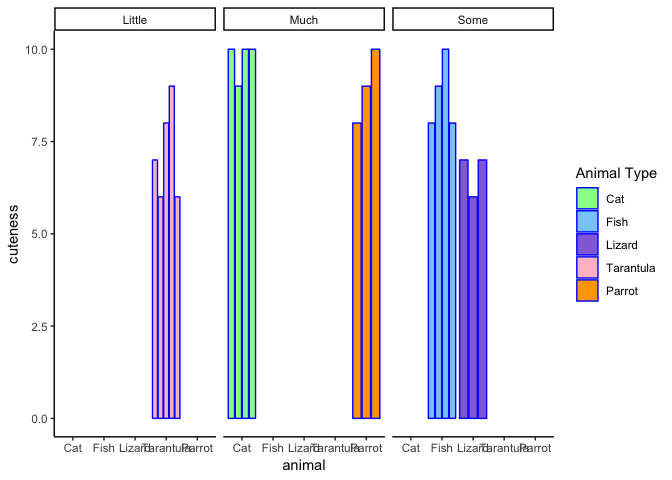
\includegraphics{FindAGene_2019_files/figure-latex/unnamed-chunk-4-1.pdf}

\section{Question 8}\label{question-8}

For question 8, we will use bio3d to search PDB for matching protein
structure files. First, we will pick the sequence with greatest
similarity to the others by asking R to generate maxima for each row in
our identity matrix.

\subsubsection{Find the most similar
sequence}\label{find-the-most-similar-sequence}

\begin{Shaded}
\begin{Highlighting}[]
\NormalTok{maxid <-}\StringTok{ }\KeywordTok{apply}\NormalTok{(alnpgrp, }\DecValTok{1}\NormalTok{, sum) }\CommentTok{# calculates the row sums; the largest ID score should indicate that it's the most similar to the others. }
\NormalTok{maxid}
\end{Highlighting}
\end{Shaded}

\begin{verbatim}
## NP_001037560.1 XP_028138990.1 XP_017886197.1 XP_014205259.1     ALN97023.1 
##          4.273          4.819          5.152          5.285          5.493 
## XP_011143830.1 XP_011344962.1 XP_011631523.1   GW790304.1_3 NP_001157188.1 
##          6.051          6.235          6.343          6.155          6.226 
## XP_012170795.1 
##          6.366
\end{verbatim}

From this, we see that XP\_012170795.1, the sequence associated with B.
terrestris, the buff-tailed bumblebee, has the most homology to the rest
of the sequences. Let's use that one to search PDB for sequence files.

\subsubsection{\texorpdfstring{Search PDB using \emph{Bombus terrestris}
PGRP protein
sequence}{Search PDB using Bombus terrestris PGRP protein sequence}}\label{search-pdb-using-bombus-terrestris-pgrp-protein-sequence}

\begin{Shaded}
\begin{Highlighting}[]
\CommentTok{# Read in the bombus sequence}
\NormalTok{bterr <-}\StringTok{ }\KeywordTok{read.fasta}\NormalTok{(}\StringTok{"bterrestris.fasta"}\NormalTok{)}
\CommentTok{# Use bio3d to run a blastp against the PDB}
\NormalTok{blastbterr <-}\StringTok{ }\KeywordTok{blast.pdb}\NormalTok{(bterr, }\DataTypeTok{database =} \StringTok{"pdb"}\NormalTok{)}
\end{Highlighting}
\end{Shaded}

\begin{verbatim}
##  Searching ... please wait (updates every 5 seconds) RID = FJYZZA57014 
##  ...................................................................
##  Reporting 30 hits
\end{verbatim}

\begin{Shaded}
\begin{Highlighting}[]
\CommentTok{# Now let's make a workable object, like a database}
\NormalTok{bterr_db <-}\StringTok{ }\KeywordTok{cbind}\NormalTok{(blastbterr}\OperatorTok{$}\NormalTok{hit.tbl}\OperatorTok{$}\NormalTok{subjectids, }
\NormalTok{                  blastbterr}\OperatorTok{$}\NormalTok{hit.tbl}\OperatorTok{$}\NormalTok{identity,}
\NormalTok{                  blastbterr}\OperatorTok{$}\NormalTok{hit.tbl}\OperatorTok{$}\NormalTok{mismatches, }
\NormalTok{                  blastbterr}\OperatorTok{$}\NormalTok{hit.tbl}\OperatorTok{$}\NormalTok{gapopens, }
\NormalTok{                  blastbterr}\OperatorTok{$}\NormalTok{hit.tbl}\OperatorTok{$}\NormalTok{evalue }
\NormalTok{                  )}
\KeywordTok{colnames}\NormalTok{(bterr_db) <-}\StringTok{ }\KeywordTok{cbind}\NormalTok{(}\StringTok{"subjectids"}\NormalTok{,}
                            \StringTok{"identity"}\NormalTok{,}
                            \StringTok{"mismatches"}\NormalTok{, }
                            \StringTok{"gapopens"}\NormalTok{,}
                            \StringTok{"evalue"}
\NormalTok{                            )}
\NormalTok{bterr_db <-}\StringTok{ }\KeywordTok{as.data.frame}\NormalTok{(bterr_db)}
\KeywordTok{head}\NormalTok{(bterr_db)}
\end{Highlighting}
\end{Shaded}

\begin{verbatim}
##   subjectids identity mismatches gapopens   evalue
## 1     4Z8I_A   51.553         76        1 4.57e-58
## 2     4ZXM_A   51.553         76        1 6.17e-58
## 3     2F2L_X   46.012         87        1 4.31e-51
## 4     1SK4_A   45.122         87        1 6.89e-47
## 5     1SK3_A   45.181         88        1 7.65e-47
## 6     1OHT_A   45.783         87        2 8.43e-47
\end{verbatim}

\subsubsection{Get background information about the
protein}\label{get-background-information-about-the-protein}

\begin{Shaded}
\begin{Highlighting}[]
\CommentTok{# Ask for the PDB annotations, }
\CommentTok{# including the stucture IDs and experimental validation info}
\NormalTok{bterrann <-}\StringTok{ }\KeywordTok{pdb.annotate}\NormalTok{(blastbterr}\OperatorTok{$}\NormalTok{hit.tbl}\OperatorTok{$}\NormalTok{subjectids)}
\end{Highlighting}
\end{Shaded}

\begin{verbatim}
## Warning in pdb.annotate(blastbterr$hit.tbl$subjectids): ids should be
## standard 4 character PDB-IDs: trying first 4 characters...
\end{verbatim}

\begin{Shaded}
\begin{Highlighting}[]
\NormalTok{bterrann}\OperatorTok{$}\NormalTok{subjectids <-}\StringTok{ }\KeywordTok{paste}\NormalTok{(bterr_db}\OperatorTok{$}\NormalTok{subjectids)}
\end{Highlighting}
\end{Shaded}

\begin{Shaded}
\begin{Highlighting}[]
\CommentTok{# Let's squish everyhting together in a big data fram}
\NormalTok{whole_bterr <-}\StringTok{ }\KeywordTok{merge.data.frame}\NormalTok{(bterrann, bterr_db)}
\CommentTok{# Quick fix to ensure R properly reads the e-value exponential notation.}
\NormalTok{whole_bterr}\OperatorTok{$}\NormalTok{evalue <-}\StringTok{ }\KeywordTok{as.numeric}\NormalTok{(}\KeywordTok{as.character}\NormalTok{(whole_bterr}\OperatorTok{$}\NormalTok{evalue))}
\end{Highlighting}
\end{Shaded}

Now we will pick out the required data from the whole merged data
frames.

\begin{Shaded}
\begin{Highlighting}[]
\NormalTok{abbrev <-}\StringTok{ }\KeywordTok{as.data.frame}\NormalTok{(}\KeywordTok{cbind}\NormalTok{(whole_bterr}\OperatorTok{$}\NormalTok{subjectids,}
\NormalTok{                whole_bterr}\OperatorTok{$}\NormalTok{compound,}
\NormalTok{                whole_bterr}\OperatorTok{$}\NormalTok{experimentalTechnique,}
\NormalTok{                whole_bterr}\OperatorTok{$}\NormalTok{resolution,}
\NormalTok{                whole_bterr}\OperatorTok{$}\NormalTok{source,}
\NormalTok{                whole_bterr}\OperatorTok{$}\NormalTok{evalue))}
\KeywordTok{colnames}\NormalTok{(abbrev) <-}\StringTok{ }\KeywordTok{c}\NormalTok{(}\StringTok{"subjectids"}\NormalTok{,}
                      \StringTok{"compounds"}\NormalTok{,}
                      \StringTok{"experimentalTechnique"}\NormalTok{,}
                      \StringTok{"resolution"}\NormalTok{,}
                      \StringTok{"source"}\NormalTok{,}
                      \StringTok{"evalue"}\NormalTok{)}
\NormalTok{abbrev}\OperatorTok{$}\NormalTok{evalue <-}\StringTok{ }\KeywordTok{as.numeric}\NormalTok{(}\KeywordTok{as.character}\NormalTok{(abbrev}\OperatorTok{$}\NormalTok{evalue))}
\CommentTok{# Fix the dumb problem with R converting evalue to a factor quick}
\NormalTok{sabbrev <-}\StringTok{ }\NormalTok{abbrev[}\KeywordTok{order}\NormalTok{(abbrev}\OperatorTok{$}\NormalTok{evalue),]}

\KeywordTok{head}\NormalTok{(sabbrev)}
\end{Highlighting}
\end{Shaded}

\begin{verbatim}
##    subjectids                                          compounds
## 24     4Z8I_A                peptidoglycan recognition protein 3
## 25     4ZXM_A PGRP domain of peptidoglycan recognition protein 3
## 14     2F2L_X   Peptidoglycan recognition protein-LC isoform LCx
## 6      1SK4_A          Peptidoglycan recognition protein I-alpha
## 5      1SK3_A          Peptidoglycan recognition protein I-alpha
## 3      1OHT_A                                    CG14704 PROTEIN
##    experimentalTechnique resolution                  source   evalue
## 24     X-RAY DIFFRACTION        2.7  Branchiostoma belcheri 4.57e-58
## 25     X-RAY DIFFRACTION        2.8  Branchiostoma belcheri 6.17e-58
## 14     X-RAY DIFFRACTION        2.1 Drosophila melanogaster 4.31e-51
## 6      X-RAY DIFFRACTION       1.65            Homo sapiens 6.89e-47
## 5      X-RAY DIFFRACTION        2.8            Homo sapiens 7.65e-47
## 3      X-RAY DIFFRACTION        2.0 Drosophila melanogaster 8.43e-47
\end{verbatim}

\section{Question 9}\label{question-9}

\begin{quote}
Generate a molecular figure of one of your identified PDB structures
using VMD. You can optionally highlight conserved residues that are
likely to be functional. Please use a white or transparent background
for your figure (i.e.~not the default black). *Based on sequence
similarity. How likely is this structure to be similar to your ``novel''
protein?
\end{quote}

From the previous question, let's select the PDB entry with the lowest
evalue: 4Z8I\_A, a peptidoglycan receptor protein origianlly
characterized in the lancelet \emph{Branchiostoma belcheri}.

\subsubsection{Get the target PDB}\label{get-the-target-pdb}

\begin{Shaded}
\begin{Highlighting}[]
\NormalTok{pgrp_pdb <-}\StringTok{ }\KeywordTok{read.pdb}\NormalTok{(}\StringTok{"4z8i"}\NormalTok{)}
\end{Highlighting}
\end{Shaded}

\begin{verbatim}
##   Note: Accessing on-line PDB file
\end{verbatim}

\begin{Shaded}
\begin{Highlighting}[]
\CommentTok{#write.pdb(pgrp_pdb, file = "bbelcheri_pgrp.pdb")}
\KeywordTok{biounit}\NormalTok{(pgrp_pdb)}
\end{Highlighting}
\end{Shaded}

\begin{verbatim}
## $`AUTHOR.determined.monomer (1 chains)`
## 
##  Call:  biounit(pdb = pgrp_pdb)
## 
##    Total Models#: 1
##      Total Atoms#: 1766,  XYZs#: 5298  Chains#: 1  (values: A)
## 
##      Protein Atoms#: 1691  (residues/Calpha atoms#: 224)
##      Nucleic acid Atoms#: 0  (residues/phosphate atoms#: 0)
## 
##      Non-protein/nucleic Atoms#: 75  (residues: 75)
##      Non-protein/nucleic resid values: [ HOH (74), ZN (1) ]
## 
##    Protein sequence:
##       QRWRSDGRCGPNYPAPDANPGECNPHAVDHCCSEWGWCGRETSHCTCSSCVDYSAGSSGT
##       CPRIVSKSEWGSRATNYNVFLSLPVPKVVIHHSAGATCSTQSSCSLQVRNIQNYHMDGRG
##       YSDIGYNFLVGNDGNVYEGRGWDRRGAHALNVNTESIGICFMGDFTSQKPTASAIAAAKS
##       LISCGVSLGKIRSGYSLYGHRDVGSTACPGNLLYDDIKSWGRYV
## 
## + attr: atom, helix, sheet, seqres, xyz,
##         calpha, call, log
\end{verbatim}

\subsubsection{View the VMD protein
gummy}\label{view-the-vmd-protein-gummy}

When I read my PMD file for the \emph{B. belcerhi} PGRP, it gives me
this cute looking gummy protein structure.
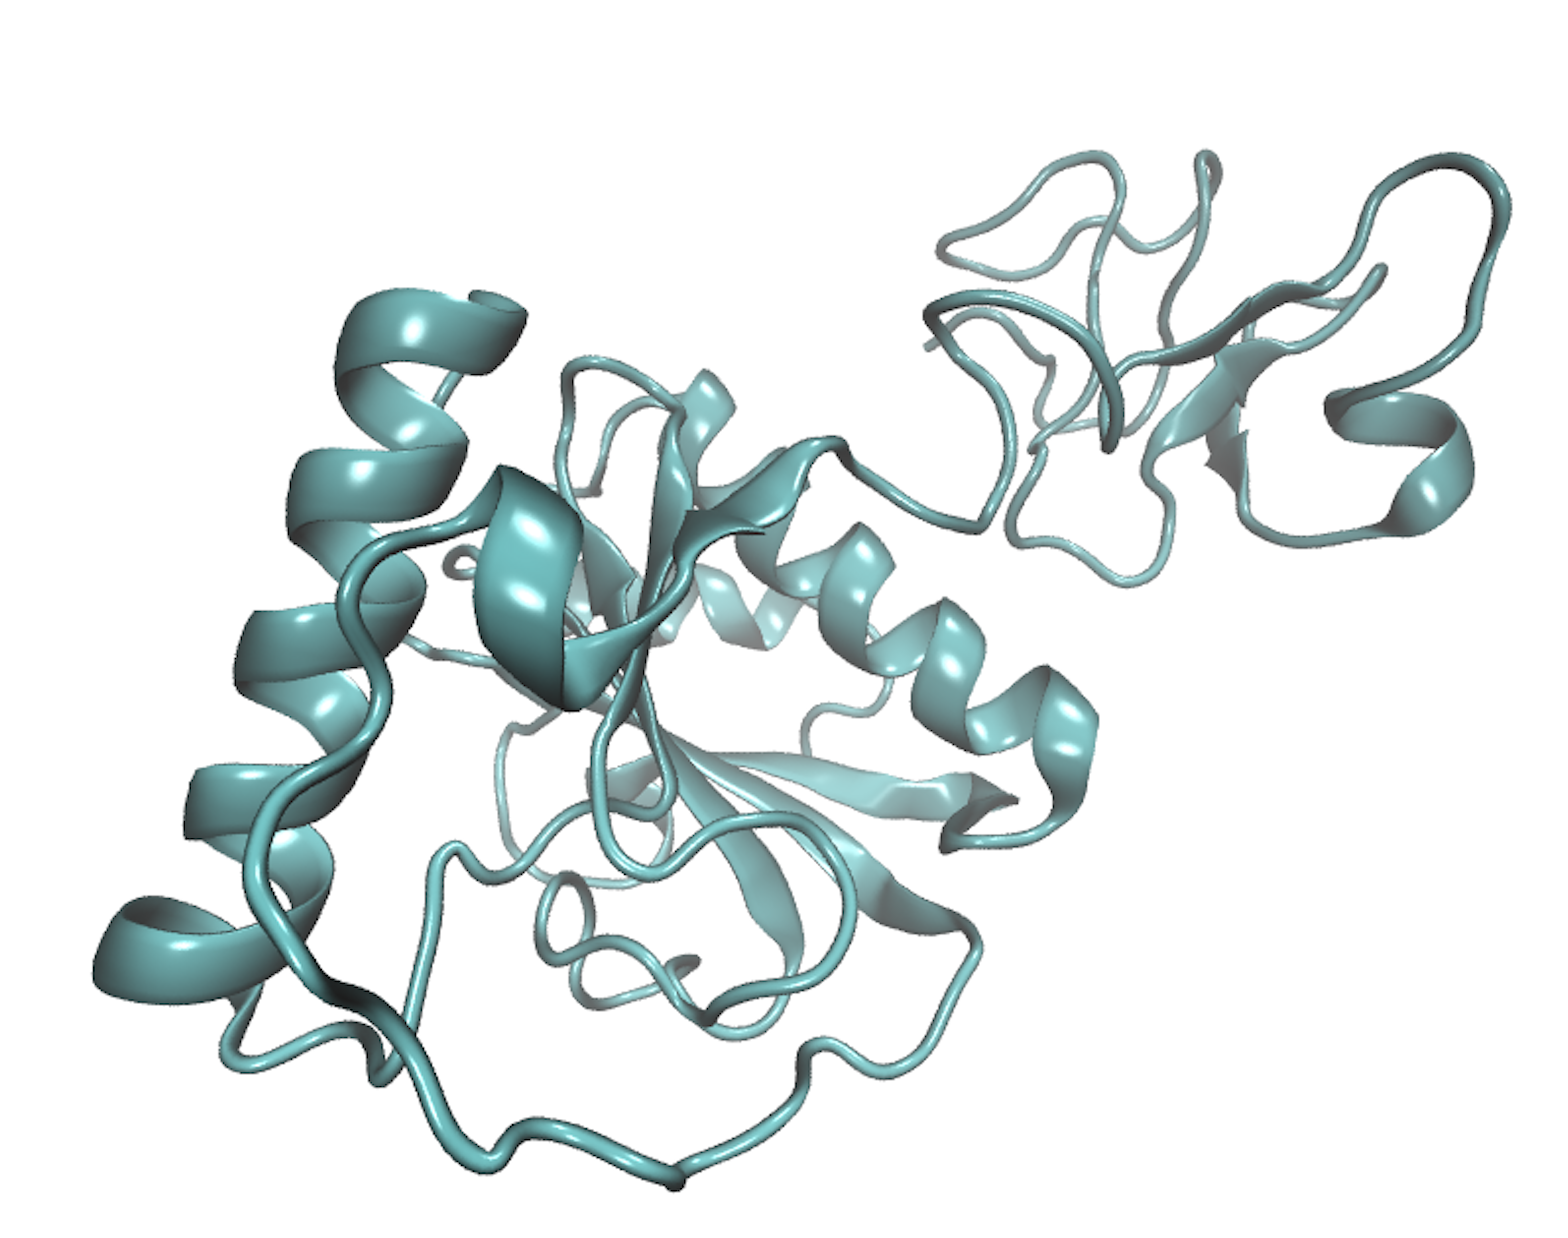
\includegraphics{q9_proteingummy_pgrp_bbelcheri.png}

\subsubsection{Probability of similar
structure}\label{probability-of-similar-structure}

I compare the sequence from \emph{V. squamosa} and \emph{B. Belcheri}
using seqaln().

\begin{Shaded}
\begin{Highlighting}[]
\NormalTok{compar <-}\StringTok{ }\KeywordTok{read.fasta}\NormalTok{(}\StringTok{"q9_aln.txt"}\NormalTok{)}
\KeywordTok{seqaln}\NormalTok{(compar)}
\end{Highlighting}
\end{Shaded}

\begin{verbatim}
##                                1        .         .         .         .         50 
## [Truncated_Name:1]GW790304.1   RMVR--------------------ATFLLVATCIA----------ICRAA
## [Truncated_Name:2]4Z8I:A|PDB   GSQRWRSDGRCGPNYPAPDANPGECNPHAVDHCCSEWGWCGRETSHCTCS
##                                   *                         *  *             *    
##                                1        .         .         .         .         50 
## 
##                               51        .         .         .         .         100 
## [Truncated_Name:1]GW790304.1   EVADSAA--TFETPNIVSRQQWGAKPPKSPTPNLKMN-PPPYVVIHHSDS
## [Truncated_Name:2]4Z8I:A|PDB   SCVDYSAGSSGTCPRIVSKSEWGSRATNY---NVFLSLPVPKVVIHHSAG
##                                   *  *  ^   * ***^  ** ^       *^ ^  * * ******   
##                               51        .         .         .         .         100 
## 
##                              101        .         .         .         .         150 
## [Truncated_Name:1]GW790304.1   VGCTTQAICQARVRSFQNDHMNSRKWNDIGYNFLVGEDGNVYEGRGWGKH
## [Truncated_Name:2]4Z8I:A|PDB   ATCSTQSSCSLQVRNIQNYHMDGRGYSDIGYNFLVGNDGNVYEGRGWDRR
##                                  *^**  *   **  ** **  * ^ ********* ********** ^^ 
##                              101        .         .         .         .         150 
## 
##                              151        .         .         .         .         200 
## [Truncated_Name:1]GW790304.1   GSHSVPYNAKSIGICLIGKFNNNVPNSASIRATQNLIAYGVANNKIKSDY
## [Truncated_Name:2]4Z8I:A|PDB   GAHALNVNTESIGICFMGDFTSQKPTASAIAAAKSLISCGVSLGKIRSGY
##                                * * ^  *  ***** ^* *  ^ *    * *   **  **   **^* * 
##                              151        .         .         .         .         200 
## 
##                              201        .         .         .        239 
## [Truncated_Name:1]GW790304.1   KLLGHRQTTKTDCPGNSLYNLIKTWPHWTDTP-------
## [Truncated_Name:2]4Z8I:A|PDB   SLYGHRDVGSTACPGNLLYDDIKSWGRYVGAAAHHHHHH
##                                 * ***    * **** **  **^* ^^            
##                              201        .         .         .        239 
## 
## Call:
##   seqaln(aln = compar)
## 
## Class:
##   fasta
## 
## Alignment dimensions:
##   2 sequence rows; 239 position columns (196 non-gap, 43 gap) 
## 
## + attr: id, ali, call
\end{verbatim}

\begin{Shaded}
\begin{Highlighting}[]
\NormalTok{alncompar <-}\StringTok{ }\KeywordTok{seqidentity}\NormalTok{(compar)}
\KeywordTok{head}\NormalTok{(alncompar)}
\end{Highlighting}
\end{Shaded}

\begin{verbatim}
##                             GW790304.1_3 4Z8I:A|PDBID|CHAIN|SEQUENCE
## GW790304.1_3                       1.000                       0.439
## 4Z8I:A|PDBID|CHAIN|SEQUENCE        0.439                       1.000
\end{verbatim}

These two sequences (GW790304.1\_3 is the \emph{V. squamosa} and
4Z8I\ldots{} is the \emph{B. belcheri}) don't appear to be very related;
they only have around \%50 identity matching. Presumably the actual
protein structure in \emph{V. squamosa} looks different. Given the
differences between immune responses in eusocial and solitary animals,
perhaps this is not as surprising?

\section{Question 10}\label{question-10}

\begin{quote}
Perform a ``Target'' search of ChEMBEL (
\url{https://www.ebi.ac.uk/chembl/} ) with your novel sequence. Are
there any Target Associated Assays and ligand efficiency data reported
that may be useful starting points for exploring potential inhibition of
your novel protein?
\end{quote}

When I search ChEMBL with the truncated \emph{V. squamosa} sequence
described in question 5, a single hit is returns. It appears to be a
n-temrinal kinase protein (or something like that) characterized in
\emph{Mus musculus}.

\begin{figure}
\centering
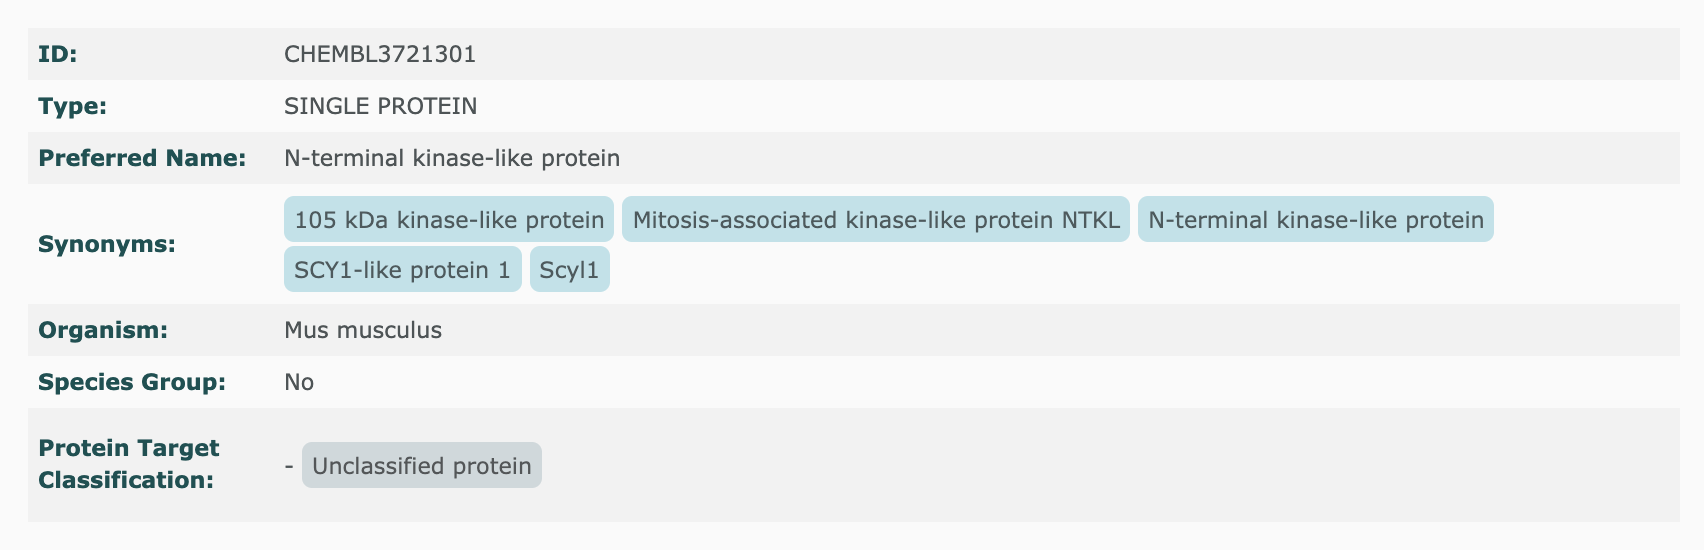
\includegraphics{q10a.png}
\caption{q10a}
\end{figure}

The majority of the functional parts of this mouse protein appear to be
associated with cellular structure, protein binding and kinase activity.
Perhaps this is reasonable to assumed for an external receptor that
interacts with the cell walls of other cells (such as bacteria or virus
capsids) 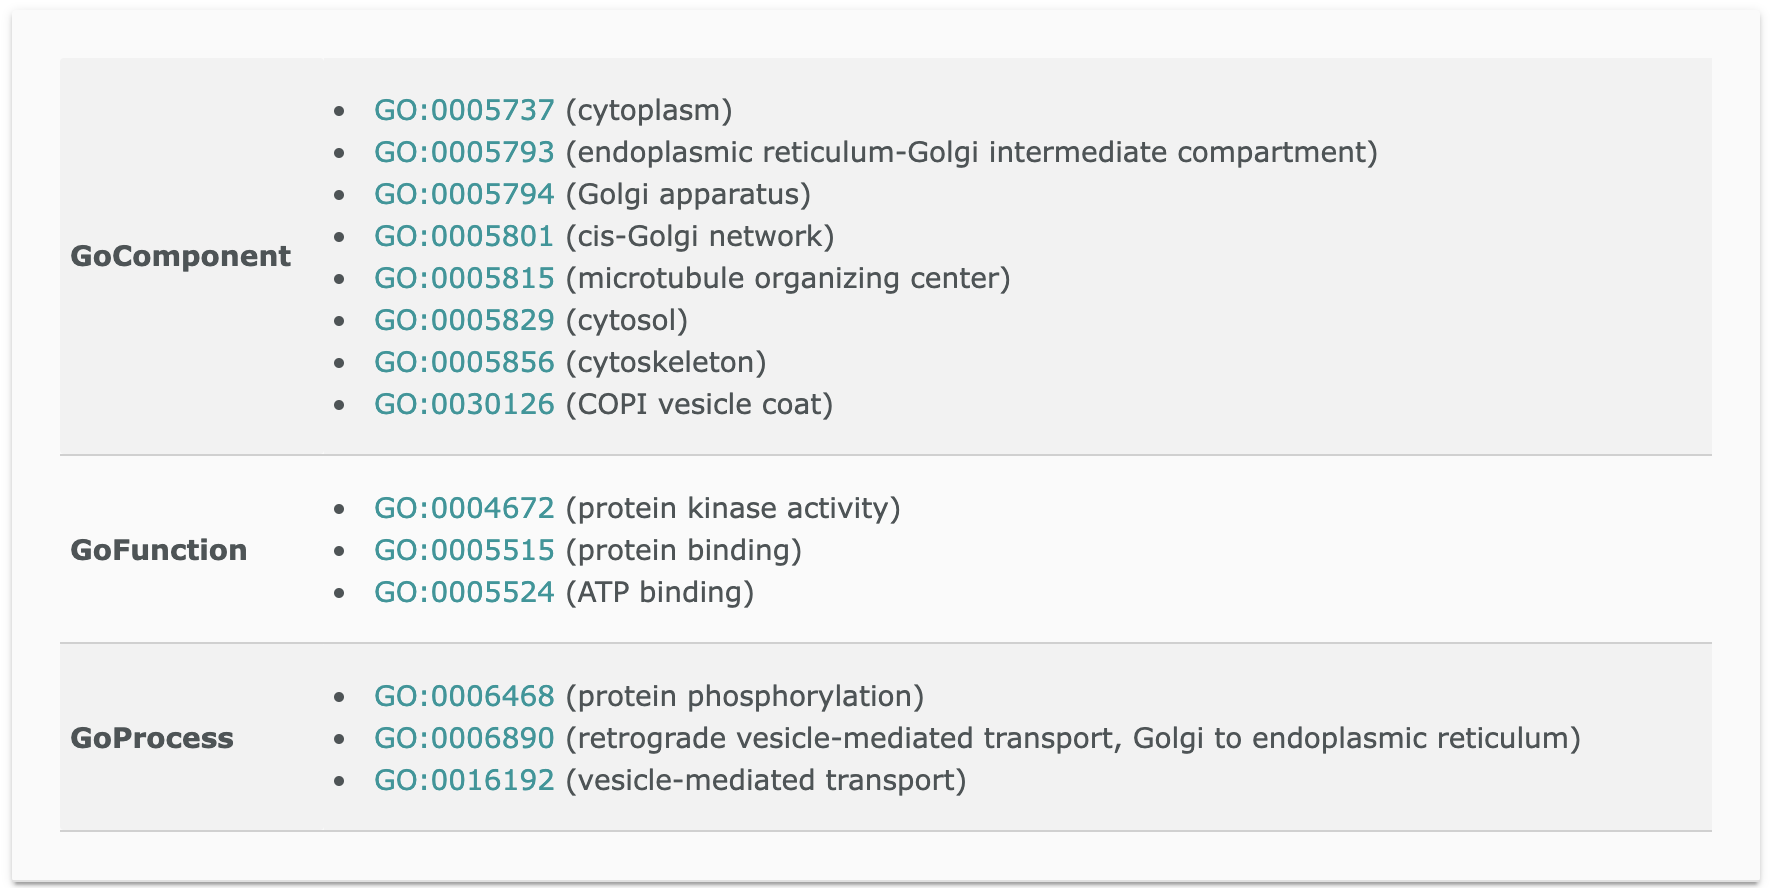
\includegraphics{q10b.png}

\section{The End}\label{the-end}

Thank you for reviewing my assignment! Hopefully it was informative!

I really appreciate this course and feel like I've learned much from it!
Thanks for your efforts in putting it together and teaching us!


\end{document}
